\documentclass[hidelinks]{scrartcl}
\usepackage{ngerman}
\usepackage[utf8]{inputenc}
\usepackage[ngerman,english]{babel}
\usepackage{amssymb}
\usepackage{graphicx}
\usepackage{fancyvrb}
\usepackage[mathbb]{}
\usepackage{amsmath}
\usepackage{amssymb}
\usepackage{float}
\usepackage{mathpazo}
\usepackage{listings}
\usepackage{pgfplots}
\usepackage{geometry}
\usepackage{upquote}
\usepackage{csquotes}
\usepackage{pdfpages}
\usepackage{colortbl}
\usepackage{rotating}
\usepackage{url}
\usepackage{hyperref}
\usepackage[nottoc]{tocbibind}
\usepackage[nomain,acronym,toc]{glossaries}
\loadglsentries{glossary}
\makeglossaries
\makeindex
\usepackage[round]{natbib}
\bibliographystyle{plainnat}
% For table highlighting and rotating of cells
\definecolor{Gray}{gray}{0.9}
\newcolumntype{g}{>{\columncolor{Gray}}c}
\newcommand*\rot{\rotatebox{90}}

\begin{document}

\pagenumbering{gobble}
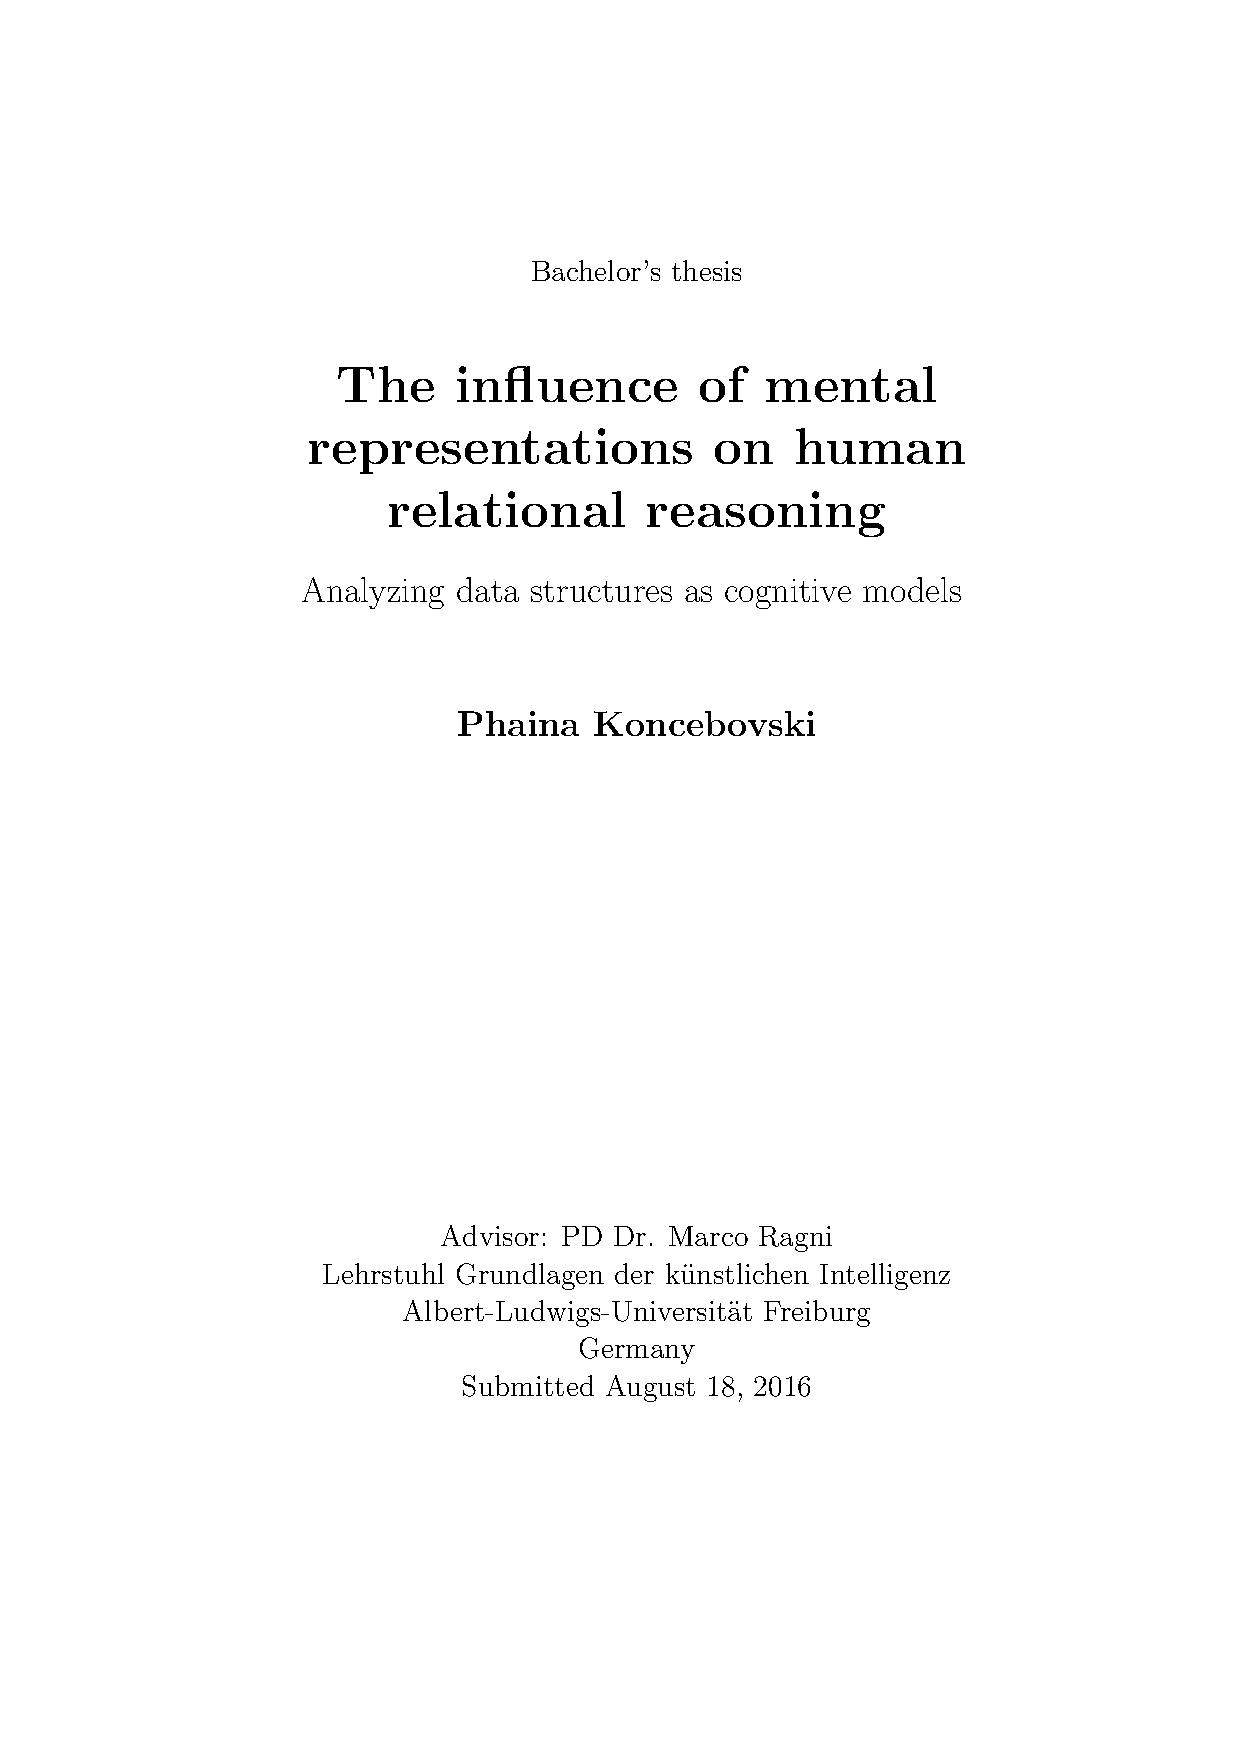
\includepdf[pages={1-}]{titlepage}
\pagenumbering{arabic}
\section*{Abstract}
\section*{Zusammenfassung}

\newpage
\tableofcontents

\newpage
%Kurze Zusammenfassung auf Deutsch
\printglossary[title=List of Terms]
\newpage

\section{Introduction (or The Cave of Mysterious Monsters)}\label{sec:introduction}
Imagine entering a mysterious cave. There are four doors, each with a combative animal behind it. You must choose a door to advance. Luckily, there's a clue:
\begin{itemize}
\label{item:initial_problem}
\item The polar bear is left of the python.
\item The alligator is right of the python.
\item The cuddly kitten is left of the python.
\end{itemize}

\begin{figure}[!ht]
	\caption{Mysterious doors}
	\label{fig:mysterious_doors}
	\centering
	
\includegraphics[width=0.7\textwidth]{Illustrations/choosing_door.jpg}
\end{figure}

Obviously, fighting against pythons, alligators and polar bears is difficult (for different reasons). You may want to choose the door with the kitten behind it. Which one is that? \\

If you only had little time to decide and no particular love for logic and statistics, it's likely that you'd choose the leftmost door.\\ 
In fact, most people would do that.
\footnote{I guess. All people I personally asked were either confused by the contrived scenario or, perhaps due to their being computer science students, immediately convinced that this was Monty Hall and they had to ``switch to the other door''.}  \\

This thesis is not (only) about human irrationality, but about spatial or \textit{relational reasoning}. Humans are born into and move through space all their life. The question of how objects are positioned in that space plays a crucial role in the ability of humans to stay alive and not constantly bump into walls. \\ Giving directions (``Turn left at the intersection immediately after the bank.''), information about where objects are located (``The box is on the table beneath the window in the room to your left.'') or remembering positions (``The quote was in the blue book on a right page somewhere at the end of the book.'') all involve relational reasoning: The ability to understand relative information as given in these sentences, interpret it correctly and - ideally - finding the object in question. \\
According to \cite{Baddeley.2007}'s model of \gls{working memory}, relational reasoning has its own dedicated space in human working memory: the so-called \textit{visuospatial sketchpad}. It holds visual and spatial information and allows mental manipulation thereof. \\

\noindent So, relational reasoning is:
\begin{itemize}
\item taking in information about space and objects in that space, 
\item taking in information about relationships between those objects and
\item drawing \gls{conclusion}s from this information.
\end{itemize}

\section{Model theory and Cognitive Basics}
Since people are able to give relations such as ``The python is left of the alligator'', when given the information from the introduction, they are obviously able to derive relations that were not explicitly given in the \gls{premise}s (i.e. deduce information). One possible way to build inferences could be by logical rules, e.g. for the transitivity \footnote{A relation is transitive ``if whenever an element a is related to an element b, and b is in turn related to an element c, then a is also related to c.'' \citep{Wikipedia.Transitive}} of relations. If \textit{A is left of B} and \textit{B is left of C}, then \textit{A is left of C}, by a simple logical rule. \\
However, this thesis is based on another way to understand human reasoning: \textit{The general theory of \gls{mental model}s} by \cite{Johnson-Laird.1986}. As summarized by \cite*{Jahn.2007}:

\begin{displayquote}
The theory of \gls{mental model}s, or the model theory for short, postulates that individuals use the meaning of assertions and general knowledge to construct models of the possibilities compatible with assertions.
\end{displayquote}

So what is stored in \gls{working memory} is not the information itself (e.g.\ as verbal representations of the \gls{premise}s), but a \textit{constructed \gls{mental model}} that represents the given information.

\cite{Goodwin.2005} extend the general theory of \gls{mental model}s to describe the domain of relational reasoning by introducing the \textit{model theory of relational reasoning}\footnote{This model theory is not to be confused with this model theory: \url{https://en.wikipedia.org/wiki/Model_theory}}. They state that
\begin{itemize}
\item models used for relational reasoning are structurally iconic, i.e.\ the relations holding between the represented entities are present in the modeled entities,
\item relational consequences are derived both from given relational information as well as general knowledge,
\item individuals construct only one, typical model and
\item ``the difficulty of an inference depends on the process of integration of the information from separate \gls{premise}s, the number of entities that have to be integrated to form a model, and the depth of the relation''.
\end{itemize}

There is considerable evidence for reasoners using the model theory for relational reasoning problems \citep{Schaeken.2007}. \\

% For abstract: Information is not represented  visually "as is", but a representative internal mental model is created.

In the case of this thesis spatial information is given in the form of \gls{premise}s. One example for a set of \gls{premise}s can be found in the introduction (see section \ref{item:initial_problem}). Individuals construct models out of the \gls{premise}s. They use these models to draw \gls{conclusion}s and determine relationships between \gls{token}s mentioned in the \gls{premise}s. \\

\citet{Johnson-Laird.1991} separate the relational reasoning process into three phases:
\begin{itemize}
\item The \textit{comprehension phase}, named the \textit{model construction phase} by \cite{Ragni.2013} in which reasoners construct a model from given information and forget the \gls{premise}s,
\item the \textit{description phase}, named the \textit{model inspection phase} by \cite{Ragni.2013}, in which reasoners inspect the mental model to derive relations that also hold but were not explicitly given in the \gls{premise}s and
\item the \textit{validation phase}, named the \textit{model variation phase} by \cite{Ragni.2013}, in which reasoners try to find alternative models in which a given \gls{conclusion} doesn't hold.
\end{itemize}

\noindent Even though the \gls{mental model}s are constructed individually, within one person, they seem to be quite predictably constructed and both stable
\begin{itemize}
\item within a population, i.e. most people construct the same internal \gls{mental model} \citep{Ragni.2013}, \citep{Knauff.2013}, \citep{Rauh.2005}
\item as well as within an individual, i.e.\ one person constructs one \gls{mental model}. \citep{Goodwin.2005}
\end{itemize}

\subsection{Inter- and Intrapersonal Stability of Mental Models}
To explain these stabilities, let's turn to the thesis advisor's work. One key idea of \cite{Ragni.2013} is the \textit{preferred model theory}.

\begin{displayquote}
A crucial assumption within our preferred model theory is that, in most situations, people only construct a single, simplified, and typical mental model and ignore all others. People are almost blind to alternative interpretations of the \gls{premise}s. We might only construct further models if the reasoning problem clearly requires us to consider alternatives. In other words, we do not think that the construction of an initial model is a stochastic process that produces one model this time and another the next time. In the preferred model theory, the construction of the initial model is, in principle, a deterministic process that always produces the same model for the same \gls{premise}s. We assume that this preferred model is the same for most people and that such preferred models bias people in a predictable way [...]. \\
\citep{Ragni.2013}
\end{displayquote}

Given the example from the introduction (see section \ref{sec:introduction} for the premises) it is both possible that the kitten is to the far left and the polar bear one door further to the right,
\begin{figure}[H]
	\caption{Kitten, Polar bear, Python, Alligator}
	\label{fig:one_ordering}
	\centering
	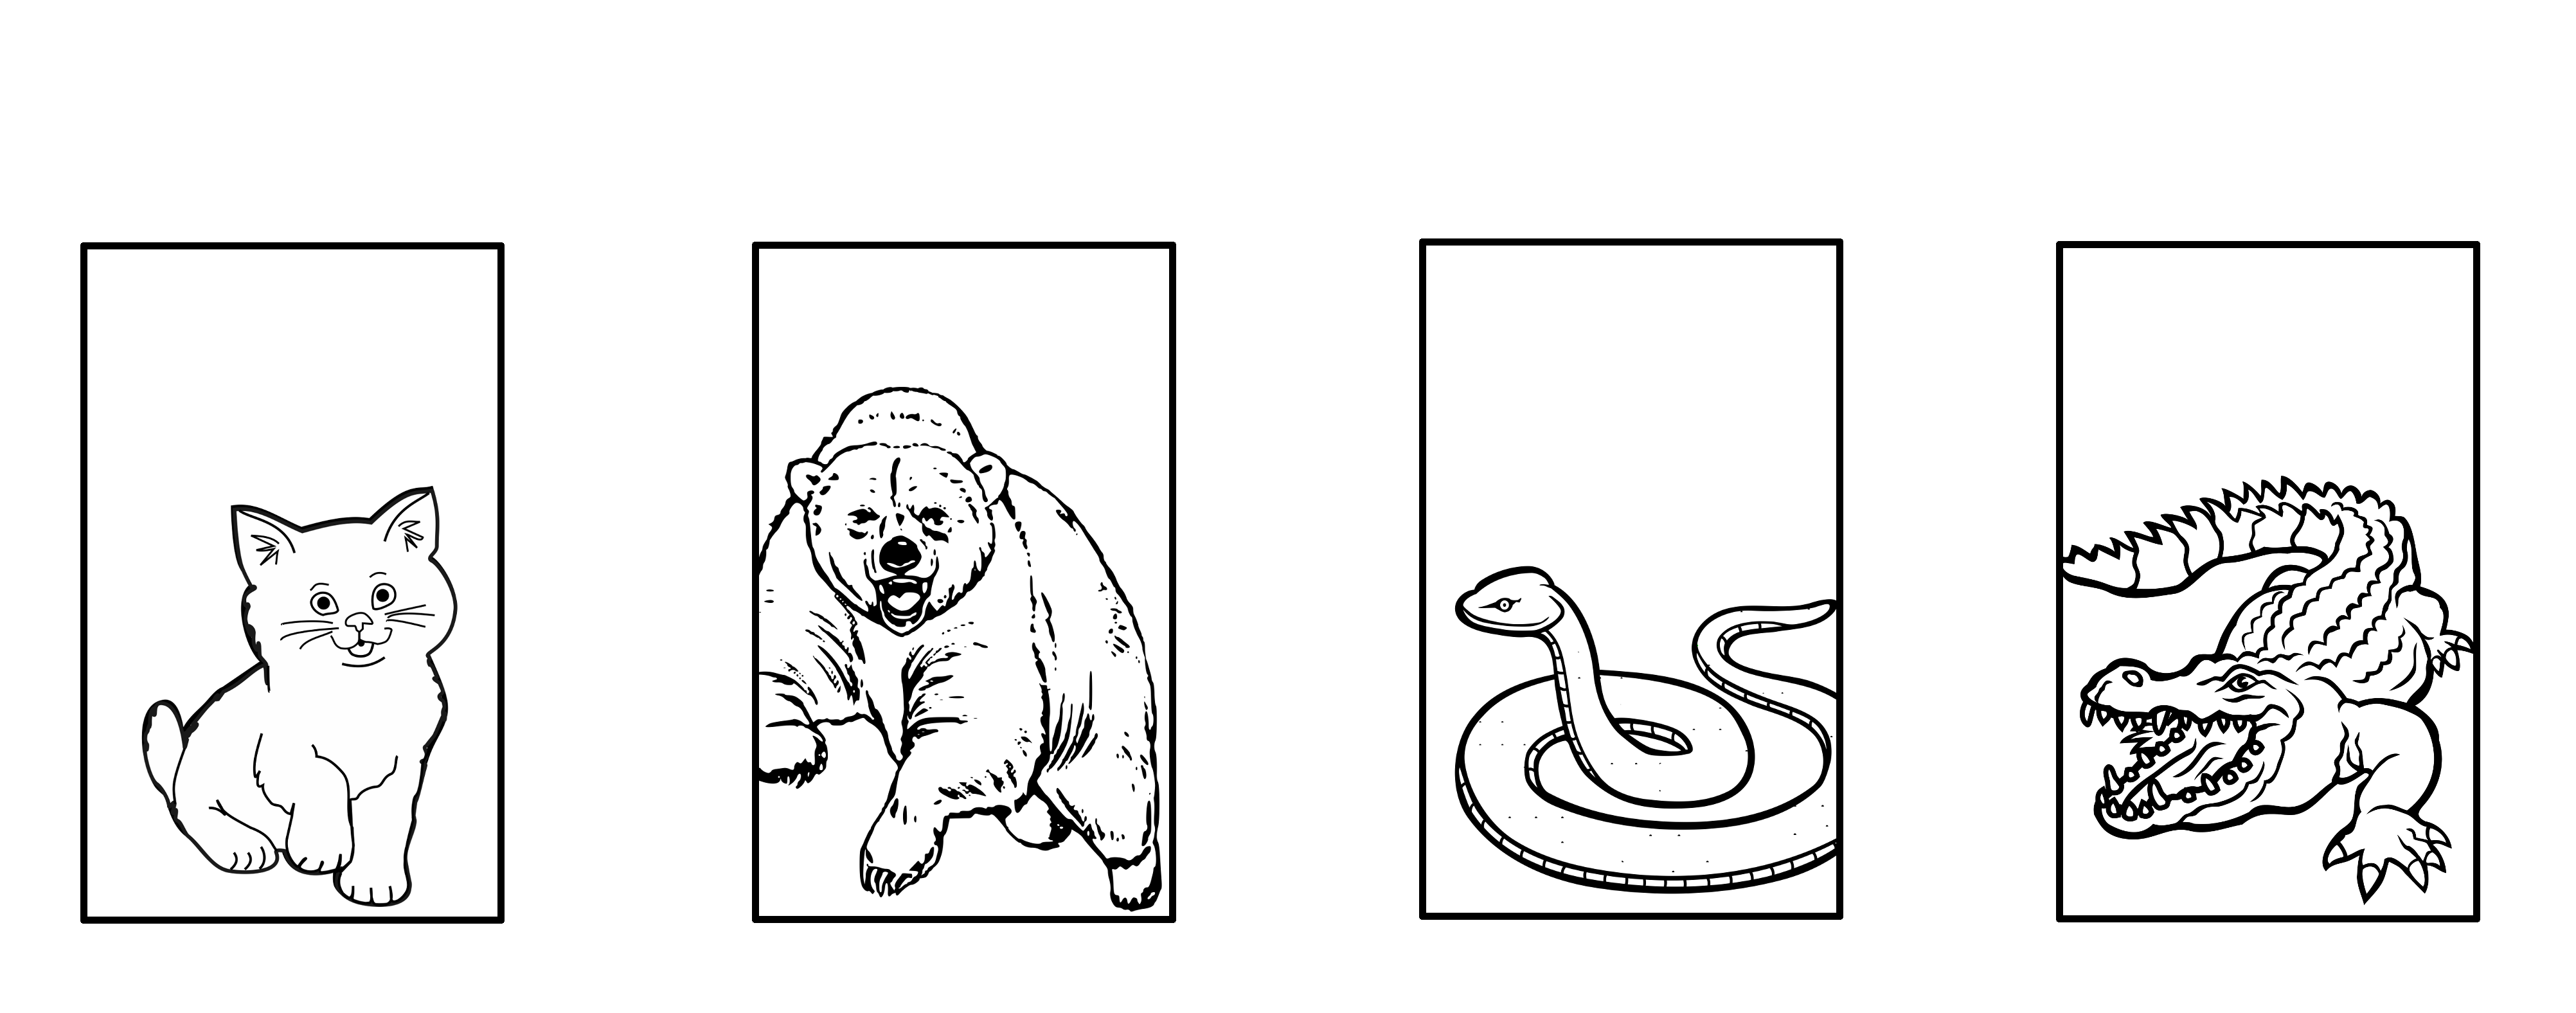
\includegraphics[width=0.8\textwidth]{Illustrations/doors_animals_1.png}
\end{figure} 

as well as them switching: The polar bear to the far left and the kitten one door further to the right.
\begin{figure}[H]
	\caption{Polar bear, Kitten, Python, Alligator}
	\label{fig:different_ordering}
	\centering
	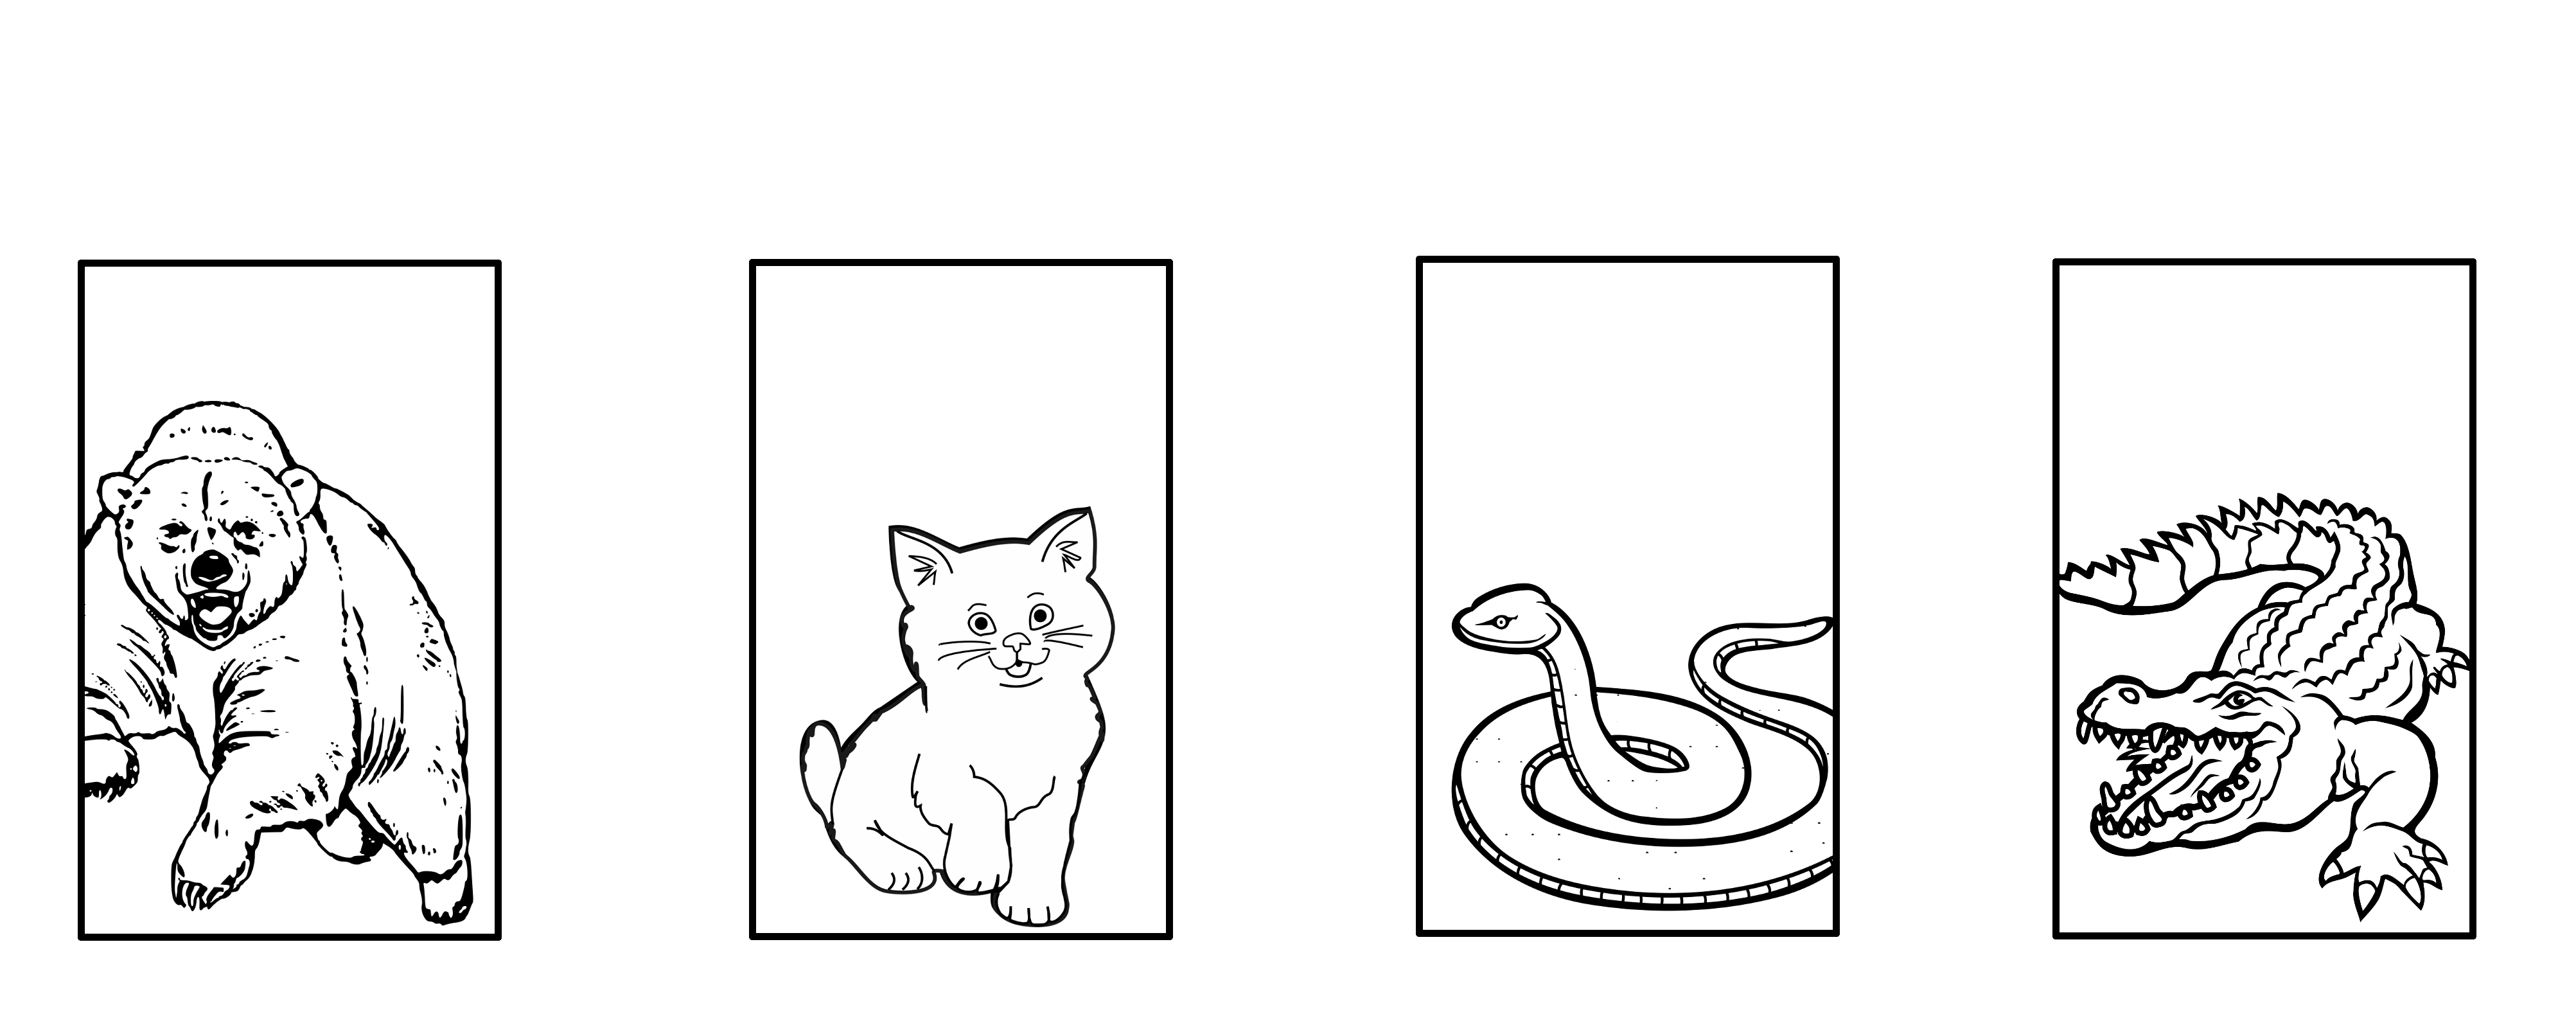
\includegraphics[width=0.8\textwidth]{Illustrations/doors_animals_2.png}
\end{figure}

When receiving new information as to what else is to the left of the python, besides the polar bear, there's a choice of ``where to put that information''. One possibility is to leave the previously constructed model of ``Polar bear, Python'' intact and to add a kitten to the left of that. The other possibility is to move the polar bear further to the left so that there's space for the kitten to crawl in between polar bear and python. \\
However, ``the preferred model is favored over others because it is easier to construct in spatial working memory'' \citep{Ragni.2013}. Moving items seems to be more work, since a moving operation requires the polar bear to be held in an extra slot, then adding the kitten in and moving the polar bear back. \cite{Ragni.2013} argue that ``preferred mental models of spatial descriptions are those constructed according to the principle that new objects are added to a model without disturbing the arrangement of those \gls{token}s already represented in the model.'' That is a variation to the description of the model construction phase by \citet{Johnson-Laird.1991} - since only one model is constructed, the \textit{preferred mental model}.

As (thereby) predicted, in an experiment by \cite{Ragni.2013} 78\% of tested individuals chose a model that was equivalently constructed to the first model for these \gls{premise}s, as shown in figure \ref{fig:one_ordering}.

This is a quite remarkable interpersonal stability, also shown by \cite{Knauff.2013} and \cite{Rauh.2005}.\\

A preferred mental model also seems to be stable within a person. If a person is presented with a different interpretation of given \gls{premise}s as the one that was constructed by the person, it seems to be very difficult to ascertain the truth of that model. Is it a correct interpretation of the given \gls{premise}s? In another experiment by \cite{Ragni.2013} participants were much slower to identify correct interpretations and more likely to reject them erroneously if they differed from the preferred mental model. Only if explicit instructions such as ``Generate all possible models'' were given, it is probable that more than one model will be constructed by an individual. ``This is a major departure from the standard model theory, which assumes that model validation always happens because people search for counterexamples to verify a putative conclusion.'' \citep{Ragni.2013}

\cite{Ragni.2013} argue that the farther removed an alternative model is from the individually constructed one it gets progressively more difficult to recognize as an also true interpretation of the \gls{premise}s.
%As a distance measure between different models, they propose local, minimal change.

\subsection{Alternative Mental Models} \label{section:alternative_mental_models}
When presenting a set of \gls{premise}s such as:

\begin{itemize}
\label{item:ambiguous}
\item The monkey is left of the bear.
\item The horse is right of the monkey.
\item The cat is left of the horse.
\end{itemize}

\noindent The preferred mental model would be:

\begin{figure}[H]
	\caption{Cat, Monkey, Bear, Horse}
	\label{fig:CMBH}
	\centering
	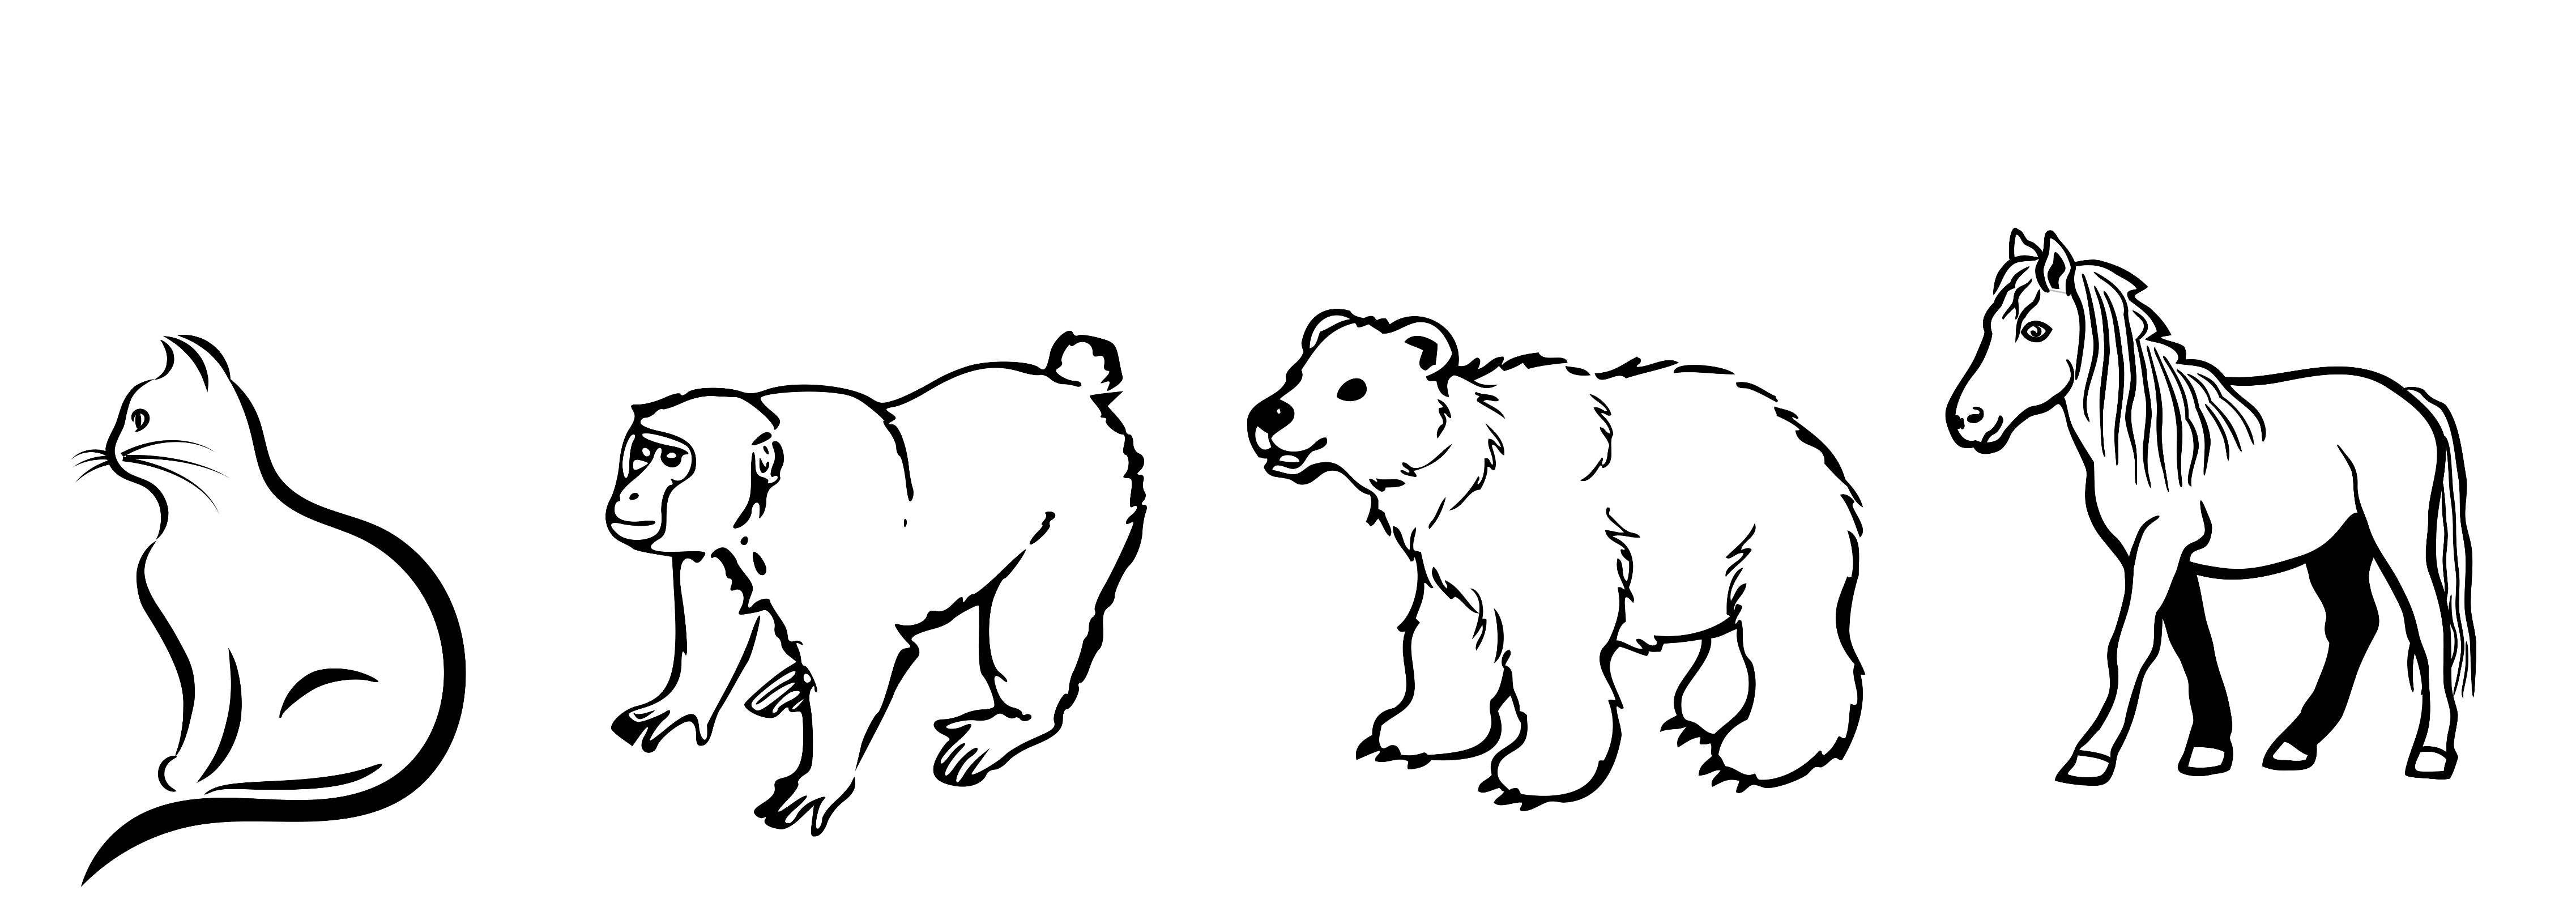
\includegraphics[width=0.8\textwidth]{Illustrations/animals_1.png}
\end{figure} 

\noindent Now, presenting people with alternative models, such as:

\begin{itemize}
\item Cat, Monkey, Horse, Bear;
\item Monkey, Bear, Cat, Horse.
\end{itemize}

the first alternative model is much more easily recognized as valid (see experiments in \cite{Ragni.2013} and \cite{Rauh.2005}) than the second one. \cite{Ragni.2013} argue that this is due to the distance between the preferred mental model and an alternative model. The smaller it is, the more likely an alternative model is recognized as valid. They write: 

\begin{displayquote}
In our theory and PRISM, this transformation distance is essential to explaining human reasoning difficulty: If an alternative model has a high transformation distance from the preferred model, it is difficult to construct and is therefore more likely to be neglected. \\
\citep{Ragni.2013}
\end{displayquote}

\noindent To determine the distance between two models, a neighborhood graph is employed.
\begin{displayquote}
In the following, we suggest using a neighborhood graph to determine the similarity between different models of a set of \gls{premise}s and, thus, the sequence in which models and alternative models are constructed. The idea is that the vertices in the neighborhood graph represent the models, and the edges connect the model with the fewest differences. Since some models are connected by fewer edges with other models, the similarity between models can be determined by the shortest path in this neighborhood graph. If a one-step transformation from one model to another model exists, then two models are called 1-nearest neighbors. In general, if two models can be connected by a minimal path of length k, then we call these two models k-neighbors. \\
\citep{Ragni.2013}
\end{displayquote}

\begin{figure}[!ht]
	\caption{Neighborhood graph for ambiguous premises}
	\label{img:neighborhood_graph}
	\centering
	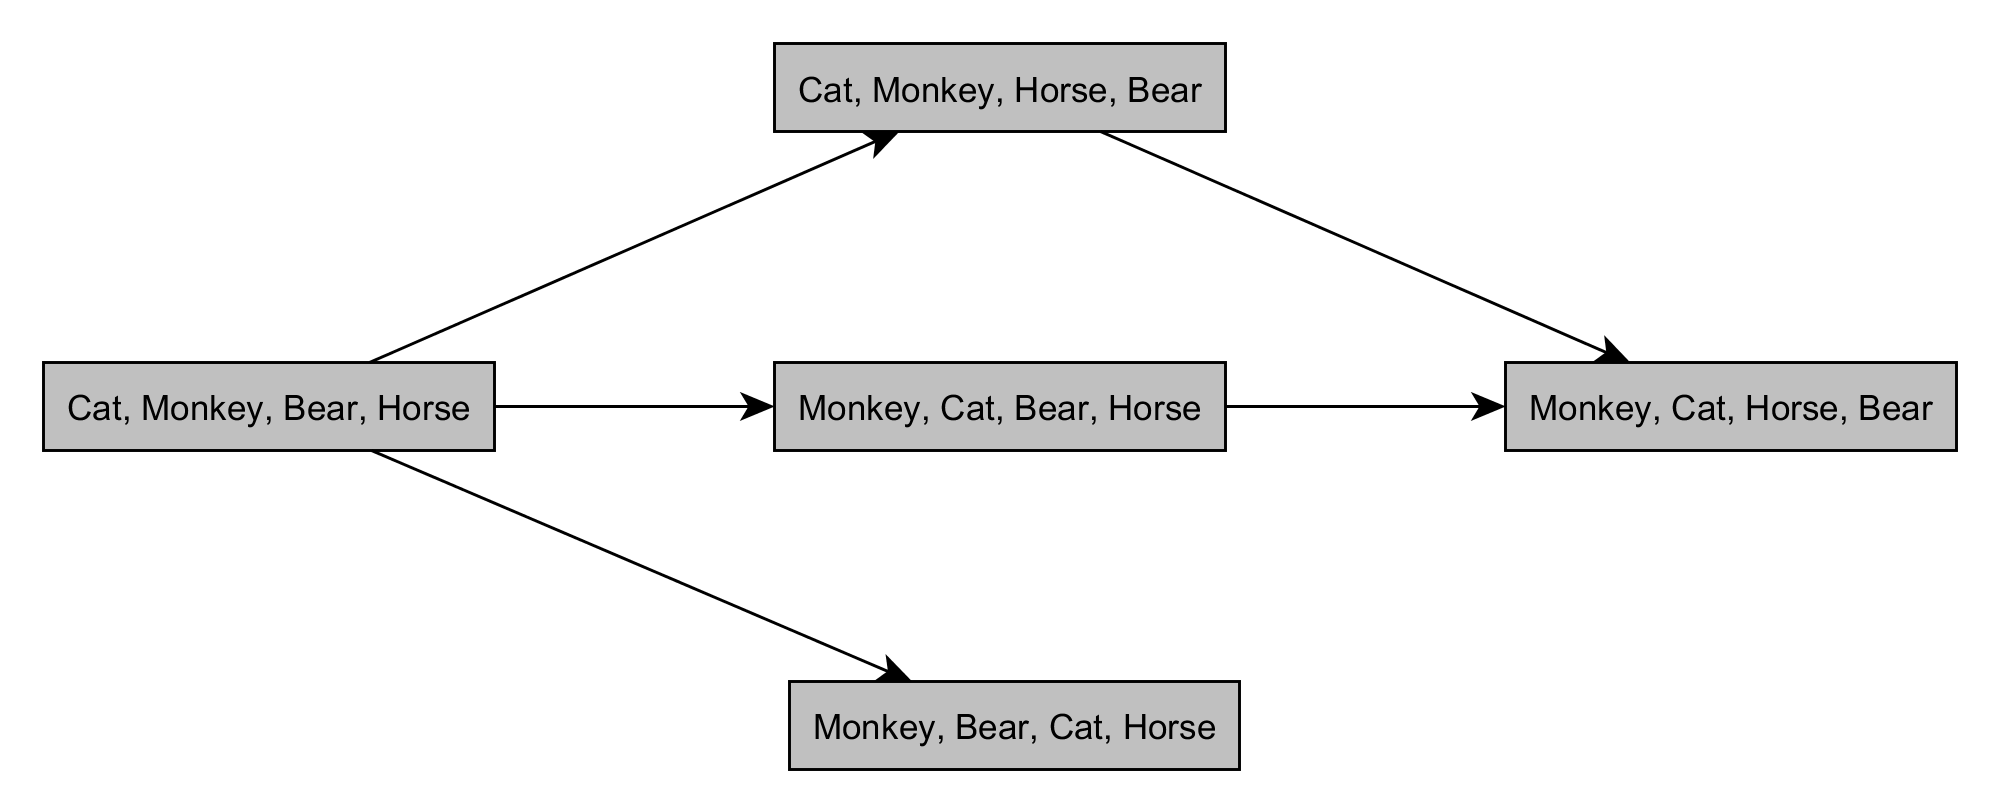
\includegraphics[width=1\textwidth]{Illustrations/neighborhood_graph.png}
\end{figure}

The leftmost model is the preferred mental model. Following an arrow to the right increases the distance to the preferred mental model. A node is gained by looking for alternative positions of tokens whose position is not determinate. Experiments by \cite{Rauh.2005} ``support the assumption of a general revision process that takes the [preferred mental model] as input and locally transforms it to come to the next alternative.''

\section{Different Classes of Problems}
A \textit{problem} designates a set of \gls{premise}s and one or more \gls{conclusion}s, which may or may not follow from the \gls{premise}s. Problems can differ in some aspects, which will be described in the following.

\subsection{Determinacy}\label{sec:determinacy}
A problem may be determinate or indeterminate. A determinate problem allows only one possible \gls{mental model} to be constructed, e.g.:
\begin{itemize}
\item The cat is left of the dog.
\item The horse is right of the dog.
\end{itemize}

\noindent An indeterminate problem allows several \gls{mental model}s to be constructed, e.g.:
\begin{itemize}
\item The cat is left of the dog.
\item The dog is right of the horse.
\end{itemize}

Indeterminate problems may be solved differently. \cite{Ragni.2013} differentiate between two strategies for inserting an ambiguous \gls{token}: The \textit{fff-strategy} (first free fit) or the \textit{ff-strategy} (first fit). In an example such as the indeterminate one above, the fff-strategy produces the preferred mental model, ``Horse, Cat, Dog''. It would first produce ``Cat, Dog'' and then insert the horse to the left of this model, producing ``Horse, Cat, Dog''. \\
The ff-strategy produces ``Cat, Horse, Dog'', an alternative model. It would insert the horse immediately to the right of the cat, shifting the dog to the right. 

\subsection{Continuity}
A problem may be continuous or discontinuous. A continuous problem gives \gls{token}s in order, e.g.:
\begin{itemize}
\item The cat is left of the dog.
\item The dog is left of the horse.
\end{itemize}

\noindent Every end \gls{token} of a \gls{premise} is the start \gls{token} of the next \gls{premise}. \\

\noindent A discontinuous problem gives \gls{token}s out of order, e.g.:
\begin{itemize}
\item The cat is left of the dog.
\item The horse is left of the dog.
\end{itemize}

\subsection{Consistency}
A problem may be consistent or inconsistent. A consistent problem gives a \gls{conclusion} that follows logically out of the \gls{premise}s. An example would be:
\begin{itemize}
\item The cat is left of the dog.
\item The dog is left of the horse.
\item Conclusion: The cat is left of the horse.
\end{itemize}

An inconsistent problem gives a \gls{conclusion} that doesn't follow logically out of the \gls{premise}s. An example would be:
\begin{itemize}
\item The cat is left of the dog.
\item The horse is left of the dog.
\item Conclusion: The cat is left of the horse.
\end{itemize}

\subsection{Difficulty}
As described in the section above, models may require different actions from the reasoner, such as inserting a new \gls{token} into a previously constructed model or evaluating the truth of a \gls{conclusion}. Obviously, problems differ from each other in the set of actions they require from the reasoner, and therefore, may also vary in their perceived difficulty and the reasoner's performance. \cite{Ragni.2013} write: ``The difficulty of an inference does not depend on the number of logically possible models but on the difficulty of mentally constructing preferred and alternative mental
models of the circumstances the premises describe.''

The question of how difficulty could be measured will be discussed in section \ref{sec:difficulty_measures}.

\section{Simulating Human Spatial Reasoning}
To understand how individuals reason and what makes a problem difficult, relational reasoning problems are carried out on a computer. For a computational implementation, a data structure has to be chosen (how to represent \gls{token}s and their relations to each other) and strategies determined, such as how to proceed if an ambiguous \gls{premise} is encountered.

\section{Previous Implementations}
Some different approaches to computationally modeling human relational reasoning will be introduced and discussed. I will limit this review to computational models that are based on the model theory by \cite{Goodwin.2005}.

\subsection{PRISM}\label{sec:PRISM}
\cite{Ragni.2013} proposed a computational model to support the preferred model theory, ``reflecting
our main assumption that people usually construct just a single, simple, and typical model but fail to consider other models in which the premises hold''. This computational model PRISM (PReferred Inferences in reasoning with Spatial mental Models) \footnote{\url{http://spatialmentalmodels.appspot.com/}} works with a data structure that is reminiscent of the tape of a Turing machine in two dimensions \footnote{\url{https://en.wikipedia.org/wiki/Turing_machine}}, in which the cells of a seemingly endless matrix are filled with \gls{token}s according to the given spatial information. A head moves from cell to cell to fill in \gls{token}s. When the \gls{premise} ``A left B'' is given, an A is written into an empty cell, the head moves one position to the right and a B is written into that cell. See figure \ref{img:PRISM} for a visual representation. 
\begin{figure}[H]
	\caption{PRISM working on \gls{premise} ``A left B''}
	\label{img:PRISM}
	\centering
	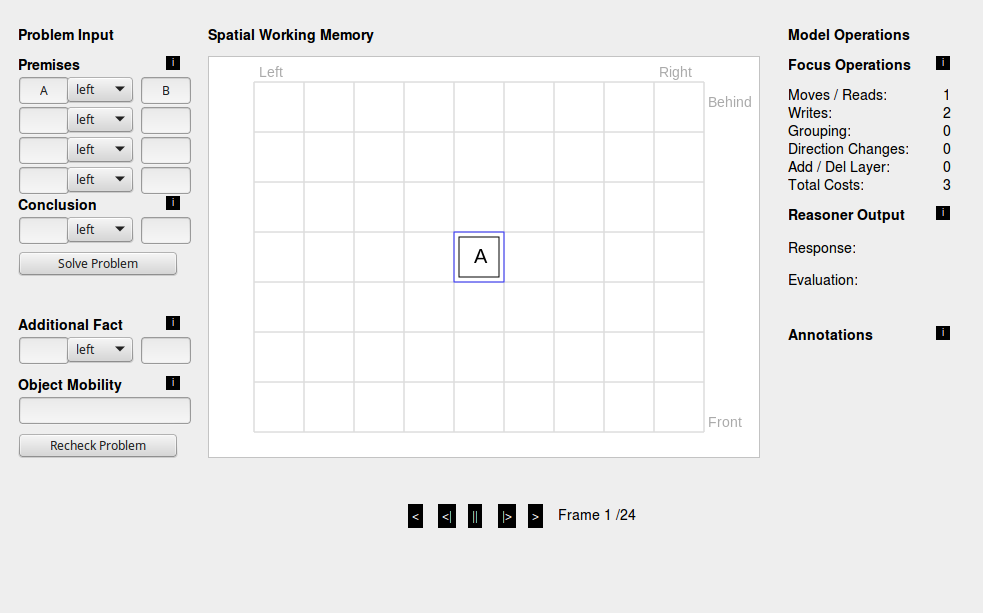
\includegraphics[width=0.77\textwidth]{Illustrations/PRISM1.png}
	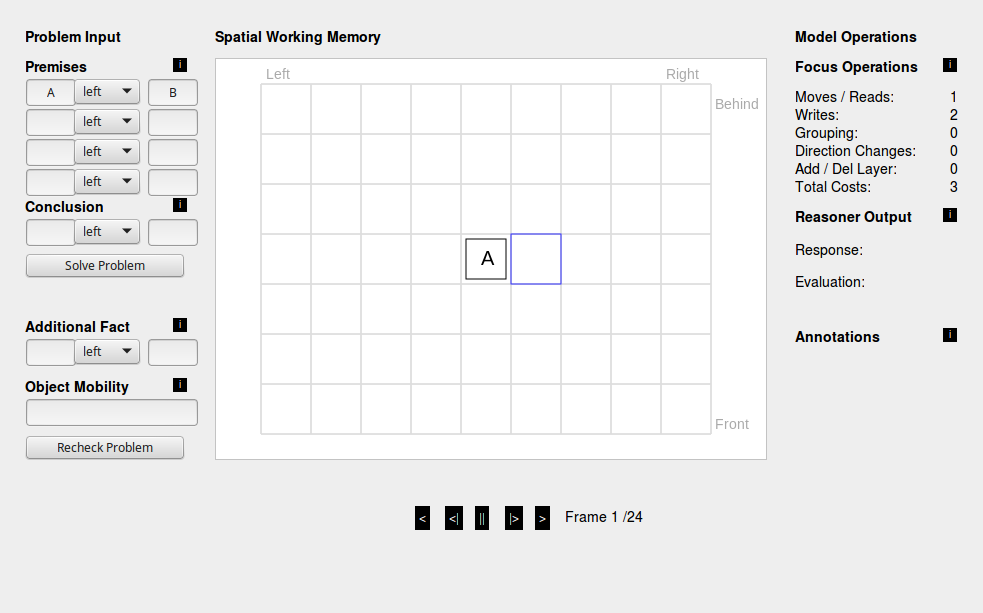
\includegraphics[width=0.77\textwidth]{Illustrations/PRISM2.png}
	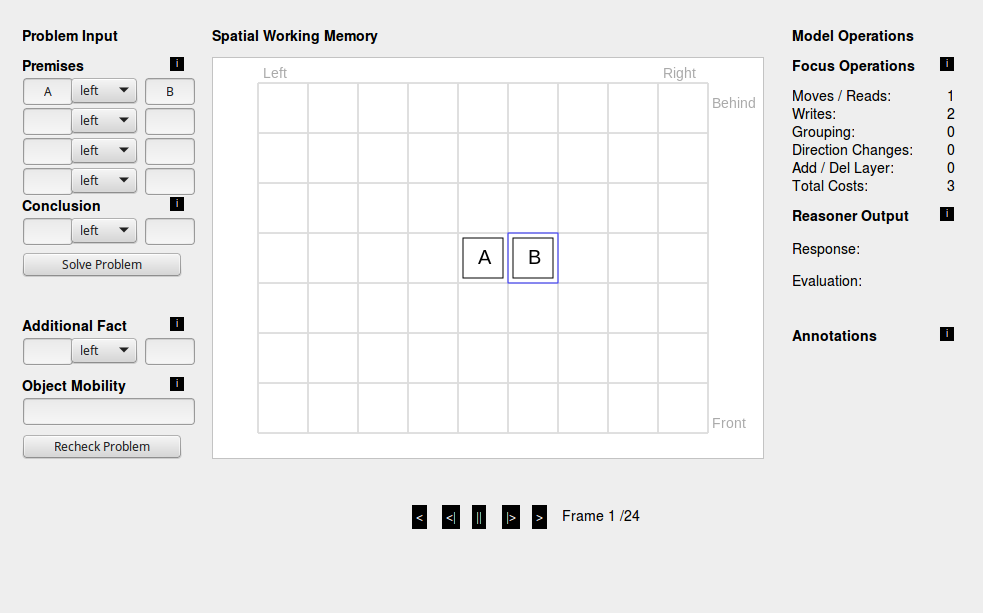
\includegraphics[width=0.77\textwidth]{Illustrations/PRISM3.png}
\end{figure}

It has widely been shown and is a generally accepted fact that human \gls{working memory} is limited in capacity \citep{Baddeley.2007}, \citep{Miller.1956}. It is very unlikely that a human reasoner is able to keep an infinite number of \gls{token}s and relations in their working memory, like PRISM is. This may be a drawback to this implementation and its utility in emulating human behavior. \\

PRISM collects information about the difficulty of a problem. This difficulty measure is based on the number of focus operations PRISM has to perform. A focus operation is the movement of the head from one cell to another. In the example ``A left B'', one focus operation is performed. In detail, the operations that PRISM counts and sums up to obtain a general difficulty measure are:

\begin{itemize}
\item Moves / Reads - Moving the head / Reading a \gls{token} in a cell,
\item Writes - Writing a \gls{token} into a cell,
\item Grouping - In the case of a merge of two models (in PRISM's case, this equates to two endless matrices that are merged into one), one of those models has to be grouped and inserted into the other, those are grouping operations,
\item Direction Changes - If a model is constructed in one direction, e.g. in the example above, it is constructed into the right direction, and an action requires the focus head to move to the other direction, e.g.\ with the \gls{premise} ``D left A'', a direction change would have occurred,
\item Add / Del Layer - If two separate models are constructed, e.g. with ``A left B'', ``C left D'', two layers are created. If those layers are then merged, e.g. with ``B left C'', one layer will be deleted.
\end{itemize}

In some experiments \footnote{\url{http://spatialmentalmodels.appspot.com/data}}, this difficulty measure correlated well with the number of test subjects who were able to correctly solve a problem. \\

PRISM deliberately chooses the fff-strategy. \cite{Ragni.2013} state that by choosing the fff-strategy, PRISM creates the preferred mental model, which most people construct and is therefore better able to emulate human performance.

\subsection{Krumnack's Linked Lists}
\cite*{Krumnack.2011} proposed viewing relational reasoning as a form of verbal reasoning, i.e. they ``assume[...] the cognitive processes in deductive reasoning to be based upon the same processes as language comprehension and generation''. They specify basic attributes of the model they assume reasoners create:

\begin{displayquote}
There exists a starting point or first object. \\
Each object is linked to the next object in the linear
order. Only the last object is not linked to other
objects. \\
While this structure has an implicit direction, the
interpretation of this direction depends on the
context.\\
\citep{Krumnack.2011}
\end{displayquote}

Computationally, they implement this model with linked lists. A linked list has a starting node, which points to another node, which points to another node, and so on, until the final node, which doesn't point anywhere. The nodes contain a link to another node and a \gls{token}. \\

When inserting a new \gls{token} into an existing linked list, they propose minimizing the amount of new links that have to be created. When inserting a new \gls{token} at the very beginning or very end of a linked list, only one new link will have to be created. This better predicts human behavior and matches the fff-strategy for inserts, as shown in an experiment in \cite{Krumnack.2011}. \\

When determining the truth of \gls{conclusion}s, it should be easier to check those models in which the \gls{token}s are named in the same order as they were named in the \gls{premise}s, because otherwise the queue has to be accessed twice: Once for finding the first \gls{token}, then accessing the queue again and searching from the beginning for the second \gls{token} mentioned in the \gls{conclusion}. This was also shown in an experiment in \cite{Krumnack.2011}. \\

Just like with PRISM, this model is unlimited in the number of \gls{token}s it accepts, which is an unlikely assumption. It also limits the order in which objects can be accessed. That is, if there's a linked list with the content ``Cat, Monkey, Bear, Horse'', evaluating ``Bear is left of Horse'' is significantly easier than evaluating ``Horse is right of Bear''. The list is only traversable in one direction (left to right). It does seem to be more difficult to traverse it ``in the other direction'', but to effectively have to start scanning the list from the beginning (Cat) seems unlikely as well.

\subsection{Bremen thingie}
Will follow...
%TODO

\section{DaStruct}
Each of these previous attempts to simulate human reasoning relied on one specific data structure. Some aspects of these data structures (e.g. the unlimited amount of \gls{token}s that can be remembered) may be unrealistic. \\
In this thesis, I will therefore analyze some competing data structures and methods and how they might relate to human relational reasoning. This computational implementation is called \textit{DaStruct} (using DAta STRUCTures for cognitive modeling).

\subsection{Implementation of DaStruct}
DaStruct was implemented in the context of this bachelor's thesis, from May 2016 to August 2016. It is implemented in Python 2.7. It is object-oriented and highly modular, allowing for free combinations of its data structures and methods. It is available under a \href{https://www.gnu.org/copyleft/gpl.html}{GPLv3} license and obtainable here: \url{https://bitbucket.org/anphisa/bachelor_thesis}. Its author is identical to the author of this bachelor's thesis.\\
%TODO check if gplv3 is a good license and make an open repository for sharing

A class diagram of DaStruct's general structure is shown in figure \ref{img:UML}. It was simplified, e.g.\ not depicting helper functions and variables.
\begin{figure}[H]
	\caption{UML class diagram for DaStruct (simplified)}
	\label{img:UML}
	\centering
	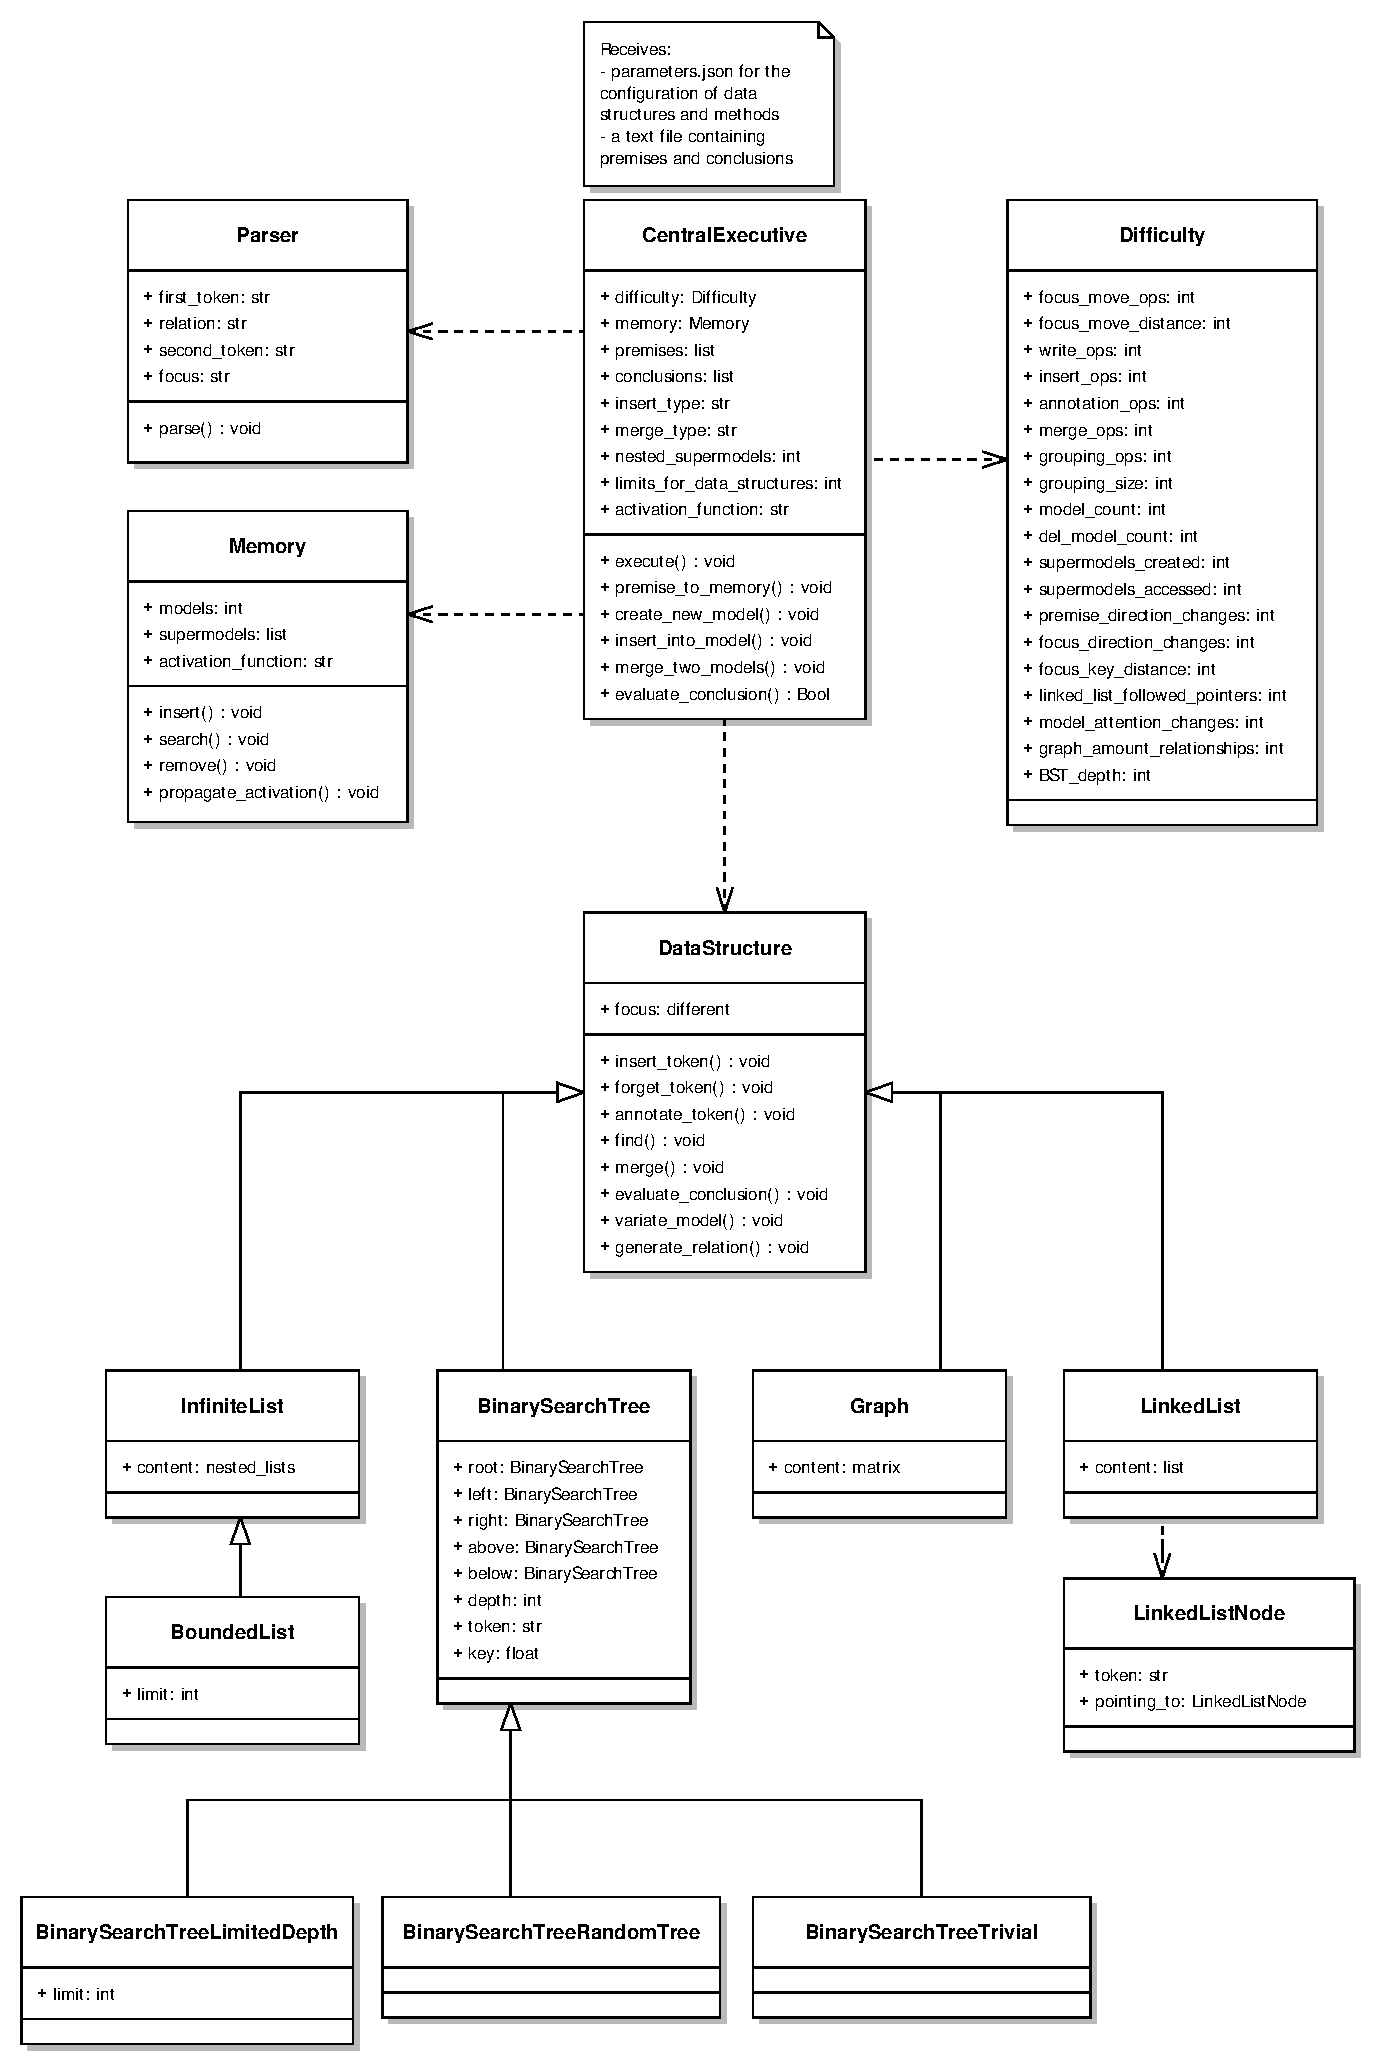
\includegraphics[width=0.95\textwidth]{Illustrations/UML_class_diagram_DaStruct.pdf}
\end{figure}

\noindent DaStruct works as follows: 

\subsubsection{Problem files}
A problem is a text file in which each line describes a \gls{premise} or a conclusion. It could look like this: 

\begin{lstlisting}[caption=A sample problem file, frame=single]
P: A left B
P: B left C
C: A left C
\end{lstlisting} 

A ``P:'' in front of a line denotes that it describes a \gls{premise}, a ``C:'' denotes a conclusion whose truth value should be determined. \\
DaStruct saves these text files with a ``.pf''-ending, short for problem file. \\
A \gls{premise} or a conclusion will always contain two \gls{token}s and a relationship between them. The relationships may be ``left'', ``right'', ``above'' or ``below''.

\subsubsection{Model construction phase}
\begin{itemize}
\item The Central Executive is instantiated. \footnote{Named after one of the components of human \gls{working memory}. In human \gls{working memory}, the central executive directs attention and chooses which information to pass on to long term memory. In this implementation, it is the master class that controls all other classes.}
\item Every line of the problem file is parsed and categorized as either a \gls{premise} or a \gls{conclusion}.
\item All \gls{premise}s are now iteratively added into models. For that, the type of the \gls{premise} is determined:
	\begin{itemize}
	\item A \textbf{type 1 \gls{premise}} is the initial \gls{premise} where both \gls{token}s have not previously been seen.
	\item A \textbf{type 2 \gls{premise}} is one where one \gls{token} has previously been seen. The other \gls{token} has to be inserted into the model of the known \gls{token}.
	\item A \textbf{type 3 \gls{premise}} is one where both \gls{token}s have not previously been seen. A new model needs to be created for this \gls{premise}. DaStruct doesn't differentiate between type 1 and type 3 \gls{premise}s.
	\item A \textbf{type 4 \gls{premise}} is one where both \gls{token}s are known. If they are part of different models, these models have to be merged.
	\end{itemize}
\item According to the \gls{premise} type, a new model is created, a \gls{token} inserted into an old one or two models are merged. In one execution of DaStruct, all models have the previously chosen same data structure type, the same insert and merge strategy.
%TODO Does this sound like it's not modular etc?
\item All models are held in memory.
\end{itemize}

\subsubsection{Conclusion Validation or Relationship Generation Phase}
\begin{itemize}
\item When all models were constructed, the \gls{conclusion}s from the problem file are validated \textit{or} relationships between given \gls{token}s are returned.
\end{itemize}

\subsubsection{Optional: Model Variation Phase}
\begin{itemize}
\item In case a conclusion was evaluated as false, the model variation phase can be entered. Analogous to \cite{Ragni.2013}, this phase is only entered if a conclusion is falsified, reflecting the belief that humans will not question it if they evaluated a conclusion as true, but might search for alternative models if they evaluated a conclusion as false. In this phase, a neighborhood graph is constructed according to which indeterminate \gls{token}s were inserted into this model. See section \ref{section:alternative_mental_models} for an explanation of the neighborhood graph.
\end{itemize}

\subsection{Data Structures}\label{sec:data_structs}
The data structures depicted in the class diagram (see image \ref{img:UML}) inheriting from the general DataStructures class will be described and explained in the following. The problem file consisting of the following \gls{premise}s:

\begin{lstlisting}[caption=Exemplary problem file, label=pf:example_pf, frame=single]
P: A left B
P: B left C
P: D above A
\end{lstlisting}

\noindent will be used as an example problem to illustrate the differing representations in different data structures.

\subsubsection{InfiniteList and BoundedList}
\textbf{InfiniteList} is a data structure that is conceptually very close to PRISM's data structure. It is made up of lists containing single layers of \gls{token}s. A \gls{token} is left of another \gls{token} if it is further to the left in the list and vice versa. \\
A layer is a 2D-structure encoding left- and right-relationships. Layers above each other encode above- and below-relationships. \\

\noindent The exemplary problem file (see listing \ref{pf:example_pf}) would yield this InfiniteList representation:

\begin{lstlisting}[caption=InfiniteList representation, label=inflist_example_pf, frame=single]
[['D', 'x', 'x'],
 ['A', 'B', 'C']]
\end{lstlisting}

The 'x's denote empty space. It is trivial to verify a conclusion, e.g.\ ``A left C''. \\

\textbf{BoundedList} is a data structure that is like InfiniteList, but contains a limit. The limit describes how many \gls{token}s may be saved in one BoundedList model at a time. E.g., given the problem file above and a BoundedList data structure with limit 2, the following three BoundedList models would represent the \gls{premise}s:

\begin{lstlisting}[caption=BoundedList representation with limit 2, label=boundedlist_example_pf, frame=single]
[['A', 'B']]

[['B', 'C']]

[['D'],
 ['A']]
\end{lstlisting}

Having constructed the first model, [['A', 'B']], the limit for \gls{token}s in this model is already filled. Therefore, when reading the \gls{premise} ``B left C'', it can not be inserted into this model anymore. A new model containing this information is created: [['B', 'C']].\\
Obviously, this limits the possibilities of evaluating conclusions. The conclusion ``A left C'' can not be verified anymore, simply because there's no model containing both the \gls{token} A as well as the \gls{token} C.

\subsubsection{BinarySearchTree, BinarySearchTreeTrivial, BinarySearchTreeLimitedDepth and BinarySearchTreeRandomTree}
Binary search trees store information in a hierarchical data structure. A tree consists of nodes, each of which contains the information to be saved in that node and a key to index the node. Every node may have up to two child nodes. A tree has a root node which is traditionally depicted at the top of the tree, making the tree ``grow downwards''. Every node may only have one parent node (or none if it is the root node). The key of a node must be bigger than its left child's key and smaller than that of its right child's key. \\

A node that is to be inserted into the tree compares its key with that of the root node: If its key is smaller, it tries an insert in the left child tree of the root tree, if its key is bigger, it tries an insert in the right child tree of the root tree. If that child tree doesn't exist yet, the node will form this child tree. If it exists, the node will further compare its key until it finds the correct free position. \\

Traditionally, binary search trees only admit left and right child nodes (and thereby a two-dimensional structure to be represented), however in the problem files ``above''- and ``below''-relations can occur. For this case, a linking of binary search trees was implemented: The root nodes of different layers (layers describing ``above''- and ``below''-layers of \gls{token}s) are linked. All child nodes of the respective root nodes are informed of the existence of this new layer and thereby all nodes of a layer. \\

\noindent The exemplary problem file (see listing \ref{pf:example_pf}) would yield this BinarySearchTree representation:

\begin{figure}[H]
	\caption{BinarySearchTree representation}
	\label{img:binarysearchtree_example_pf}
	\centering
	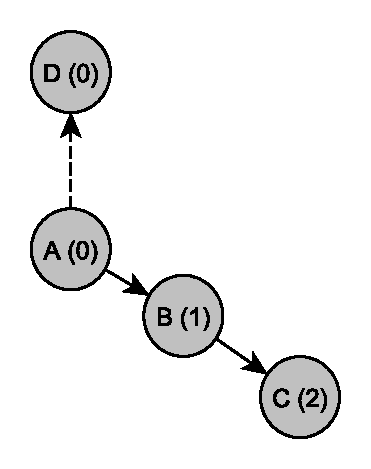
\includegraphics[width=0.3\textwidth]{Illustrations/BinarySearchTree.pdf}
\end{figure}

The nodes are drawn as circles, the keys indexing the nodes are in brackets after the \gls{token}s. The \gls{token}s A and D have the same key since they are in different trees (just linked with the ``above''-relation). Tokens A and B have no left children, therefore no nodes to the left. \\
The data structure \textbf{BinarySearchTree} implements a binary search tree as described. \\

The \textbf{BinarySearchTreeTrivial} data structure differs only in the insert-procedure from the normal BinarySearchTree data structure. Trees support intelligent procedures such as the rotation of leaves (to free up space), which BinarySearchTreeTrivial doesn't support. \footnote{This was rather a stage in development of the BinarySearchTree data structure than an individual idea. It worked well enough, which is why it was included in the tests.} \\

The \textbf{BinarySearchTreeLimitedDepth} data structure has a depth limit, i.e.\ inserts node only to a given depth of the tree. The depth of a tree describes the distance of the furthest child node to the root node of a tree. E.g.\ with depth limit 2, the exemplary problem file (see listing \ref{pf:example_pf}) would yield this representation:

\begin{figure}[H]
	\caption{BinarySearchTreeLimitedDepth representation}
	\label{img:binarysearchtreelimiteddepth_example_pf}
	\centering
	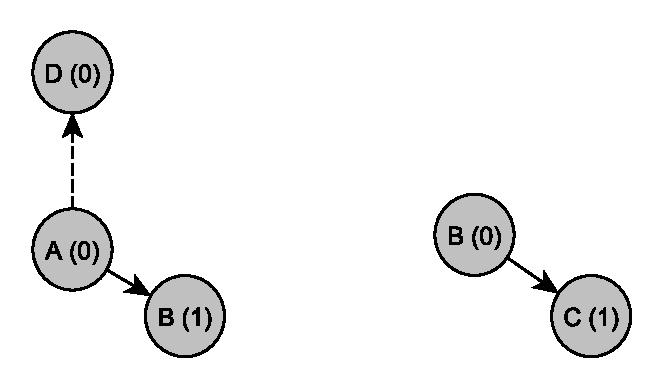
\includegraphics[width=0.5\textwidth]{Illustrations/BinarySearchTreeLimitedDepth.pdf}
\end{figure}

The \gls{token} D can still be inserted into the first model since it doesn't increase the depth of either tree to a depth larger than 2. However, the second \gls{premise} ``B left C'' will yield its own tree (with own key numbering as well, so the \gls{token} B has different keys in the two models). There is no alternative place to insert the \gls{token} C into the first model: As \gls{token} A's left child, it would be evaluated as being left of \gls{token} B, which is incorrect. \\

The \textbf{BinarySearchTreeRandomTree} data structure builds a random binary search tree at each insert. Inserting \gls{token}s not by the order in which they ``arrived'' but randomly may even out the height of the tree. E.g. inserting keys 1, 2, 3, 4, 5, 6 in this order will yield a tree that is not very balanced. Inserting the same keys in a randomized order, e.g.\ as 3, 5, 1, 6, 2, 4 will yield a much more even tree.

\begin{figure}[H]
	\caption{Two binary search trees containing numbers from 1 to 6}
	\label{img:random_tree}
	\centering
	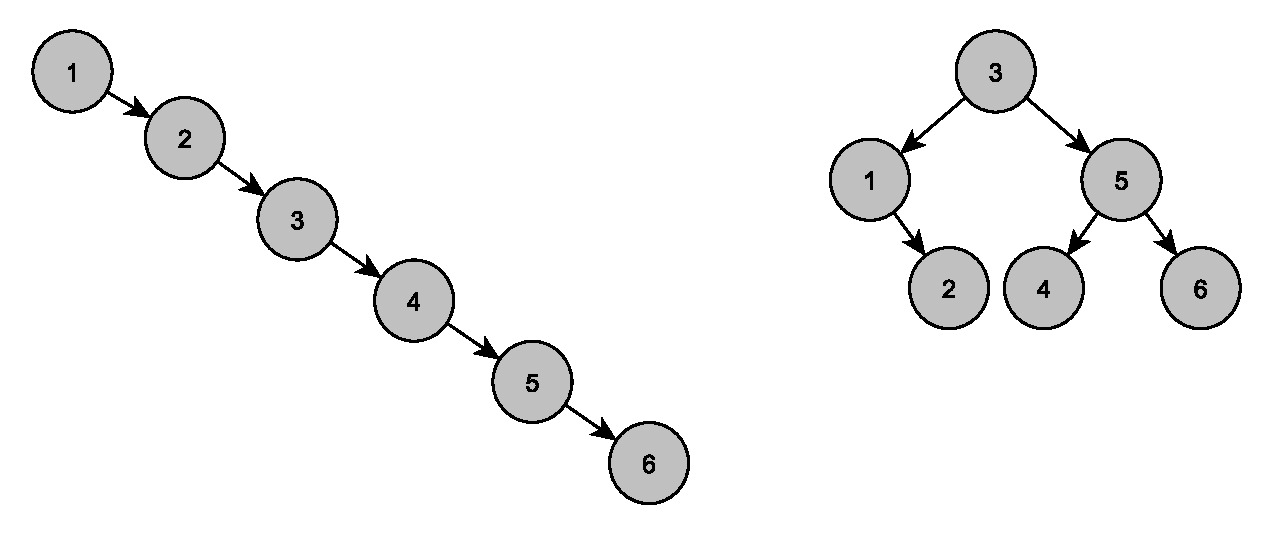
\includegraphics[width=0.9\textwidth]{Illustrations/BinarySearchTreeRandomTree.pdf}
\end{figure}

To this end, the BinarySearchTreeRandomTree has an InfiniteList data structure at its base. Into this structure, it inserts all the \gls{token}s from the \gls{premise}s. For every layer in the InfiniteList, it assigns a key linearly: The leftmost object receives key 1, the next key 2, etc. Then, choosing the items from the list randomly, it inserts the objects into a BinarySearchTree structure. \\
In this case, it would construct the same structure as InfiniteList (see listing \ref{inflist_example_pf}) and then assign key values. The assignation of key values is shown in table \ref{tab:random_search_tree_keys}.

\begin{table}[H]
\caption{Key assignment for random search tree} 
\label{tab:random_search_tree_keys}
\centering
	\begin{tabular}{c c}
	Token 	& Key value \\
	D		& 1 \\
	\hline
	A		& 1 \\
	B		& 2 \\
	C		& 3
	\end{tabular}
\end{table}

After first constructing a binary search tree just for \gls{token} D, it would construct a binary search tree and insert \gls{token}s A, B and C in a random order.

\subsubsection{Graph}
A graph stores information visually. A graph for the exemplary problem file (see listing \ref{pf:example_pf}) might look like this:

\begin{figure}[H]
	\caption{Graph representation}
	\label{img:graph_example_pf}
	\centering
	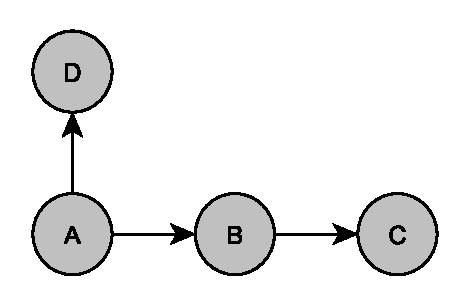
\includegraphics[width=0.4\textwidth]{Illustrations/Graph.pdf}
\end{figure}

Other forms could be imagined, e.g.\ without arrows indicating the relationship between \gls{token}s, or a representation that isn't based on a grid-like structure. DaStruct doesn't allow for ambiguous relationship (as in a non grid-like structure).\\

A \textbf{Graph} model with the information from the exemplary problem file (see listing \ref{pf:example_pf}) would have this internal representation:

\begin{lstlisting}[caption=Graph representation, label=graph_example_pf, frame=single]
[['',  'A', 'B', 'C', 'D'],
 ['A', 'x', 'l', 'l', 'b'],
 ['B', 'r', 'x', 'l', 'x'],
 ['C', 'r', 'r', 'x', 'x'],
 ['D', 'a', 'x', 'x', 'x']]
\end{lstlisting}

This representation represents an adjacency matrix \footnote{An adjacency matrix represents a graph by indicating which nodes are adjacent to each other, i.e.\ linked by an edge. In DaStruct, additionally the type of relationship between nodes (\gls{token}s) is specified.}. The first row and the first column contain the \gls{token}s which are contained in the model. The cells between them contain their relation. If the relation between B and C should be generated or evaluated, the row beginning with \gls{token} B and the column beginning with \gls{token} C will be chosen. The cell at their intersection describes the relation between B and C: 'l', short for left. \\
All other relations are similarly abbreviated. An 'x' denotes no recorded relationship.

\subsubsection{LinkedList}
The \textbf{LinkedList} data structure was implemented analogously to \cite{Krumnack.2011}'s implementation of linked lists. LinkedLists are lists similar to the InfiniteList implementation, however they only support access in one direction (left to right). A linked list is a list of LinkedListNodes.
A LinkedListNode structure contains a \gls{token} and a pointer. If it is to the left of another node, its pointer will point to that node. If it is the rightmost node, its pointer won't point to another node. \\

The ``outer list'' that LinkedListNodes are contained in is necessary to enable three-dimensional indexing. Nodes that come first in the list are above nodes that come later in the list. \\
The outer list of LinkedListNodes for the exemplary problem file (see listing \ref{pf:example_pf}) would look like this:

\begin{lstlisting}[caption=LinkedList representation, label=linkedlist_example_pf, frame=single]
['D', 'A']
\end{lstlisting}

\noindent Expanding the nodes, it would look like this:

\begin{lstlisting}[caption=Expanded LinkedList representation, label=exp_linkedlist_example_pf, frame=single]
['D', 'A' -> 'B' -> 'C']
\end{lstlisting}

The arrows denote a pointer from one node to another.

\subsection{Data Methods and Additional Features}\label{sec:data_methods}
All data structures can freely be combined with different methods for treating the \gls{token}s and \gls{premise}s. Methods can describe different strategies for certain operations (such as inserts or merges), limit the size of a data structure or the memory strength of DaStruct.

\subsubsection{Insert strategy}
A type 2 \gls{premise}, i.e. one where one \gls{token} is known and present in at least one model and the other \gls{token} is unknown, needs an insert procedure. In the exemplary problem file (see listing \ref{pf:example_pf}) the first \gls{premise} ``A left B'' builds a model ``A, B'', the second \gls{premise} ``B left C'' now requires an insert of \gls{token} C into the previously constructed model ``A, B''. In this case the insert is deterministic and yields the model ''A, B, C''. However, for indeterminate inserts a strategy needs to be chosen. DaStruct supports the ff- and fff-strategy for inserts. For an explanation of these inserts, see section \ref{sec:determinacy}.

\subsubsection{Merge strategy}\label{sec:merge_strategy}
A type 4 \gls{premise}, i.e. one where both \gls{token}s are known, but part of different models, requires a merge of these models. DaStruct supports two merge strategies: \\

\textbf{Integrate merge} \\
The integrate merge integrates two models into one model. Both single models will be deleted and a new model containing the merged information will be inserted into memory. \\

\textbf{Supermodel merge} \\
The supermodel merge will create supermodels instead of integrating models into one. This problem file:

\begin{lstlisting}[caption=Problem files for merges, label=pf_merging, frame=single]
P: A left B
P: C left D
P: E left F
P: B left C
P: D left E
\end{lstlisting}

would yield this hierarchy of supermodels:

\begin{figure}[H]
	\caption{Supermodel merge}
	\label{img:supermodel_merge}
	\centering
	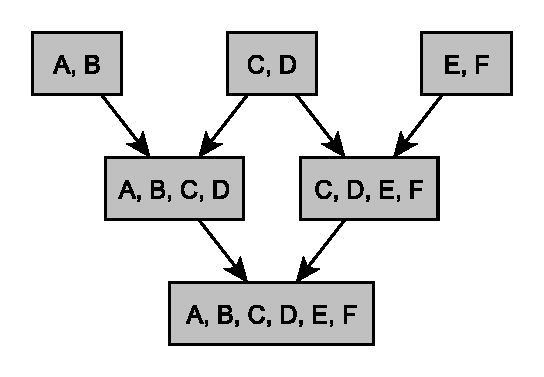
\includegraphics[width=0.6\textwidth]{Illustrations/supermodel_merge.pdf}
\end{figure}

The models on top are the models that represent the \gls{premise}s 1-3. Premises 4 and 5 specify the required merge operations. When performing the merges, the three models on top combine to the two supermodels on the second layer of the image. These two supermodels can again be combined to the supermodel of supermodels on the third layer of the image. \\
DaStruct has the option to limit the depth to which supermodels will be created. If that limit was set to 1 for the example above, the first layer of supermodels would still be constructed, the one below wouldn't. The \gls{premise} ``A left F'' would then be evaluated as false. If the limit was set to 2, the second layer of supermodels would be constructed and the \gls{premise} ``A left F'' would be evaluated as true.

\subsubsection{Distance on the neighborhood graph}
When \gls{premise}s call for indeterminate inserts, several models are possible representations of those \gls{premise}s. See section \ref{section:alternative_mental_models} for an explanation for how and when alternative mental models may be constructed. DaStruct has an optional limit for the distance on the neighborhood graph that an alternative model may have to the preferred mental model.

\subsubsection{Activation function}\label{sec:activation_function}
In neural networks \footnote{Computer systems inspired by the structure of biological neural networks, e.g.\ constructed similarly to the human visual system.}, activation functions serve as an analogue to the rate of action potential of a cell, i.e. the ``likelihood of a neuron firing''. In DaStruct, the activation function describes the process of forgetting information. \\
In 1885, Hermann Ebbinghaus started testing his own memory: He memorized sheets of nonsense syllables and tested his remaining knowledge at certain points in time \citep{Ebbinghaus.1913}. The resulting \textit{forgetting curve} describes how many of these syllables he could still remember at a given point in time. Extrapolating his data, the function
\begin{gather}
R = e^{(-t/S)}
\end{gather}
is an approximation of his forgetting curve. R is the amount of information that was retained, t is the point in time after the learning of the information and S is a factor that describes the ``memory strength''. Increasing it will increase the amount of information that is remembered at a given point in time. \\

This curve is the basis for some activation functions that were used in experiments with DaStruct. The forgetting of \gls{token}s was modeled, not the forgetting of relations between \gls{token}s. Tokens are somewhat similar to Ebbinghaus' syllables since in the experiment they had names such as A, B or C and were therefore presumably not considerably more meaningful to participants than Ebbinghaus' random syllables. Ebbinghaus' curve describes the process of forgetting a set of syllables and therefore one chunk of information. For DaStruct, it was interesting to model the forgetting of several \gls{token}s that are not related to each other. \\

\cite*{Yffelti.2016} proposes a function that works on the basis of Ebbinghaus' forgetting curve when several pieces of information are added into a memory system. In DaStruct's case, the time points of insertion of a \gls{token} into memory were set as the \gls{premise} number in which a \gls{token} was first seen. It is assumed that every \gls{token} has the same strength of insertion, so no \gls{token} is inserted more strongly than other \gls{token}s. In that case, \cite{Yffelti.2016} propose the following formula based on the superposition principle\footnote{\url{https://en.wikipedia.org/wiki/Superposition_principle}}:
\begin{gather}
I(t) = \Delta I \cdot \sum \limits_{i=1}^n  e^{-\frac{t-i \cdot \Delta t}{S}} \cdot \theta(t - t_i),
\end{gather}
where 
\begin{equation}
  \theta(t)=\begin{cases}
               1, ~~t \geq 0, \\
               0, ~~t < 0
            \end{cases}
\end{equation}
is the Heaviside function \footnote{\url{https://en.wikipedia.org/wiki/Heaviside_step_function}}. \\

For different memory strength factors $S$, this function is shown plotted in figures \ref{fig:Equidistant equiintense information injections into a system with memory strength 1} and \ref{fig:Equidistant equiintense information injections into a system with memory strength 2}.

\begin{figure}[H]
\centering
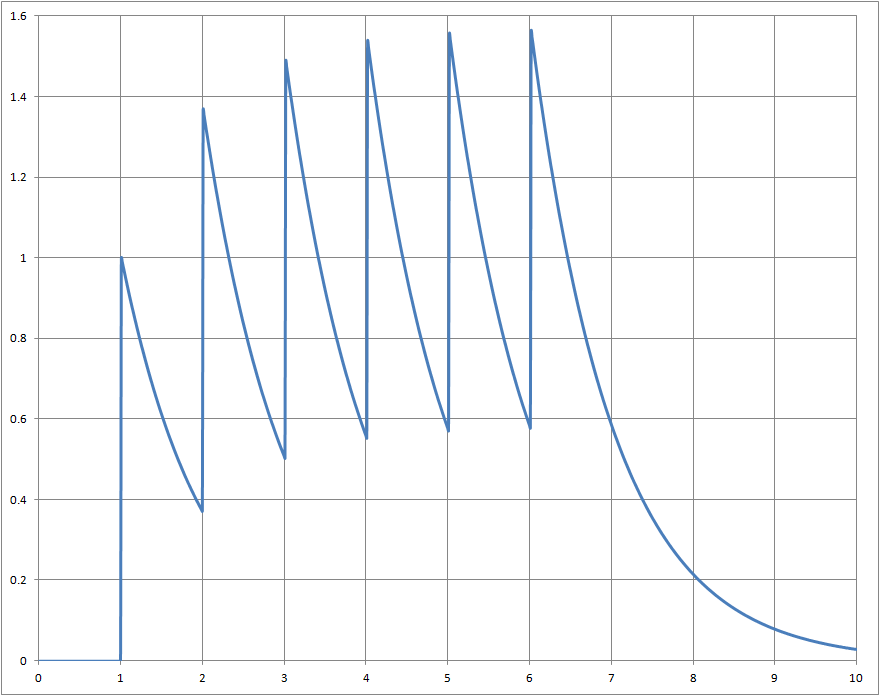
\includegraphics[width=0.7\textwidth]{Illustrations/Equidistant_equiintense_with_S=1.png}
\caption{Equidistant information injections with equal intensities ($\Delta I_i = 1$) into a system with memory strength $S=1$.}
\label{fig:Equidistant equiintense information injections into a system with memory strength 1}
\end{figure}

\begin{figure}[H]
\centering
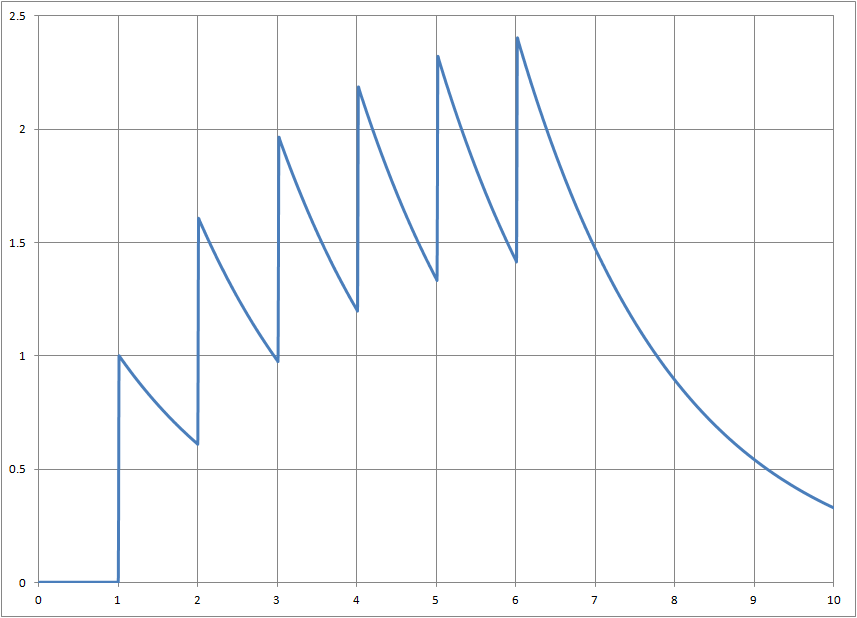
\includegraphics[width=0.7\textwidth]{Illustrations/Equidistant_equiintense_with_S=2.png}
\caption{Equidistant information injections with equal intensities ($\Delta I_i = 1$) into a system with memory strength $S=2$.}
\label{fig:Equidistant equiintense information injections into a system with memory strength 2}
\end{figure}

For DaStruct, I used the upper values of this function with memory strengths 2 and 3 to obtain a limit that denotes which \gls{token}s are forgotten again, assuming that \gls{token}s that were seen the longest ago are forgotten first. In practice, with this problem file:

\begin{lstlisting}[caption=Premise file, frame=single]
P: A left B
P: B left C
P: D above A
\end{lstlisting}

This is the table denoting the time step at which each \gls{token} was first seen:

\begin{table}[H]
	\begin{tabular}{| c c |}
	\hline
	Time step 	& Token \\
	1			& A		\\
	1			& B		\\
	2			& C		\\
	3			& D		\\
	\hline
	\end{tabular}
	\caption{At which time step tokens were first seen}
\end{table}

Tokens A and B were both seen in the first \gls{premise} and thereby time step 1. The function given by \cite{Yffelti.2016} yields the following results for each time step:

\begin{table}[H]
	\begin{tabular}{| c c |}
	\hline
	Time step 	& Result of \cite{Yffelti.2016}'s function with memory strength $S$ = 2	\\
	1			& 1											\\
	2			& 1.6065									\\
	3			& 1.9646									\\
	\hline
	\end{tabular}
	\caption{At which time step \gls{token}s were first seen}
\end{table}

In DaStruct, this result was used as a limit. That is, at time step 2 all \gls{token}s that were seen in a time step smaller than 1.6065 are forgotten. This would mean that \gls{token}s A and B are not accessible anymore. The premise ``B left C'' would now be categorized as a type 1/type 3 premise instead of a type 2 premise.

\subsection{Difficulty Measures and Cumulated Difficulty Measures}\label{sec:difficulty_measures}
While processing the \gls{premise}s and conclusion, DaStruct collects a variety of difficulty measures. PRISM collected some difficulty measures (see \ref{sec:PRISM} for a description of these), DaStruct aims to obtain a higher resolution of measures. \\
The difficulty measures that were collected were chosen 
\begin{itemize}
	\item for the fact that they were easily implementable, e.g.\ if implementing them followed naturally out of their computational implementation,
	\item for the fact that a similar (or the same) difficulty measure was implemented in PRISM,
	\item for the fact that the author assumed that they would measure difficulty.
\end{itemize}
This exemplary problem set will help illustrate the difficulty measures collected by DaStruct:

\begin{lstlisting}[caption=Exemplary problem file, label=pf:example_pf_diff_measures, frame=single]
P: A left B
P: B left C
P: E right D
P: D right C
\end{lstlisting}

The explanations of difficulty measures are based on an unlimited data structure. The results of the measures will vary for limited data structures.

\subsubsection{Collected Difficulty Measures}
The following single difficulty measures were collected by DaStruct:

\begin{itemize}
	\item \textbf{Focus move operations}: Measures whether the focus was moved at all. The focus is 		analogous to PRISM's head movements (see section \ref{sec:PRISM} for those). The focus is always 		moved to the last \gls{token} that was important. When considering the exemplary problem file (see listing \ref{pf:example_pf_diff_measures}), for the first premise one focus move operation would be performed. First, the \gls{token} A would be inserted into the model and the focus would be on \gls{token} A. Immediately thereafter, \gls{token} B would be inserted and focus would be shifted to it. For premise 2, the focus would be shifted from \gls{token} B to \gls{token} C. In premise 3, the focus is shifted from \gls{token} E to \gls{token} D, for premise 4 no focus move operation is necessary since in both the models that are merged the focus lies on the \gls{token}s that describe the merge operation.\\
	Altogether, the exemplary problem file has 3 focus move operations.
	\item \textbf{Focus move distance}: Measures how far the focus was moved. In the exemplary problem file (see listing \ref{pf:example_pf_diff_measures}), every focus move operation only moves the focus for distance 1. If the distance between \gls{token}s is bigger, the focus move distance increases. E.g.\ given the \gls{premise}s ``A left B'', ``B left C'' and ``D left A'', the focus would have to move from \gls{token} C to \gls{token} A for the third premise. The move distance of that move operation would be 2.\\
	Altogether, the exemplary problem file has a focus move distance of 3.
	\item \textbf{Focus key distance}: Measures the key distance when performing a focus move operation in a BinarySearchTree. When the node in focus changes in a BinarySearchTree, this measure collects the key distance between them. \\
	Altogether, the exemplary problem file has a focus key distance of xxx, when utilizing the base data structure BinarySearchTree.
	%TODO
	\item \textbf{Write operations}: Measures the amount of write operations. When no merge operations are required, this equates to the number of \gls{token}s that are mentioned. If a merge operation is required and the merge strategy is set to integrate, one set of \gls{token}s need to be ``rewritten'', i.e.\ integrated into another model. This increases the write operation measure to a number higher than the number of \gls{token}s mentioned. In the exemplary problem file (see listing \ref{pf:example_pf_diff_measures}), the model ``D, E'' needs to be inserted into the model ``A, B, C'' on the basis of the premise ``D right C''. 5 write operations were performed up to this point. If the merge strategy is set to integrate, the model ``D, E'' would need to be rewritten, thus creating the merged model ``A, B, C, D, E''.\\
	Altogether, the exemplary problem file requires 7 write operations if the merge strategy is set to integrate and 5 if the merge strategy is set to supermodel.
	\item \textbf{Insert operations}: Measures the amount of insert operations. For a type 2 \gls{premise}, a \gls{token} needs to be inserted into an existing model. \\
	Altogether, the exemplary problem file requires one insert operation. The first and third \gls{premise} are type 1/type 3 \gls{premise}s and do not specify an insert. The fourth \gls{premise} is a type 4 \gls{premise}. Only the second \gls{premise} is a type 2 \gls{premise} and requires one insert operation.
	\item \textbf{Merge operations}: Measures the amount of merge operations. For a type 4 \gls{premise}, two models need to be merged. \\
	Altogether, the exemplary problem file requires one merge operation, as specified in the fourth \gls{premise}.
	\item \textbf{Supermodels created}: Measures the amount of supermodels that were created. If a merge is performed, this increases the amount of supermodels. For the example in \ref{sec:merge_strategy}, this would be 3. \\
	Altogether, the exemplary problem file would, if executed with the supermodel merge strategy, require one supermodel to be created.
	\item \textbf{Supermodels accessed}: Measures the amount of supermodels that needed to be accessed. If a conclusion is to be evaluated, supermodels are checked going iteratively deeper into the hierarchy of supermodels. How many supermodels needed to be checked to verify a conclusion is what is measured here. If a conclusion is inconsistent, all supermodels are accessed. \\
	Altogether, the exemplary problem file requires no supermodels to be accessed.
	\item \textbf{Grouping operations}: Measures the amount of times the content of a model is grouped for a merge operation. In preparation for a merge operation, the entire content of a model is grouped. \\
	Altogether, the exemplary problem file requires one grouping operation.
	\item \textbf{Grouping size}: Measures the size (in amount of \gls{token}s) that were grouped for a merge. In the case of the exemplary problem file (see listing \ref{pf:example_pf_diff_measures}), the second model is merged into the first model. The second model is grouped. It contains two \gls{token}s. \\
	Altogether, the exemplary problem file requires a grouping of size 2.
	\item \textbf{Premise direction changes}: Measures how often the relationship that is specified in the premises changes. In the exemplary problem file (see listing \ref{pf:example_pf_diff_measures}), the first two \gls{premise}s contain the relationship ``left'', while the second two \gls{premise}s contain the relationship ``right''. This change is measured. \\
	Altogether, the exemplary problem file has one premise direction change.
	\item \textbf{Focus direction change}: Measures how often the direction of the focus changed. Every time a focus move operation occurs, the focus moves into a direction. E.g.\ in the first \gls{premise} of the exemplary problem file (see listing \ref{pf:example_pf_diff_measures}), the focus moves from \gls{token} A to \gls{token} B. Since \gls{token} A is left of \gls{token} B, the focus moves into the direction right. That direction stays the same for \gls{premise} two. In \gls{premise} three, no change of focus direction occurs, since ``E right D'' is the initial \gls{premise} for a new model. Since \gls{premise} four does not require any focus move operation, there's no focus direction change required. \\
	Altogether, the exemplary problem file has no focus direction changes.
	\item \textbf{Linked List followed a pointer}: Measures how often a pointer was followed in a LinkedList data structure. \\
	Altogether, the exemplary problem file requires xxx pointers to be followed.
	%TODO
	\item \textbf{Model attention changes}: Measures how often the attention changes from one model to another. In the exemplary problem file (see listing \ref{pf:example_pf_diff_measures}), the first two \gls{premise}s describe one model. The third \gls{premise} instantiates a new model. The attention is shifted to this second model. The fourth \gls{premise} describes a merge. The attention is shifted to the newly created merged model. \\
	Altogether, the exemplary problem file requires 3 model attention changes.
	\item \textbf{Annotation operations}: Measured how often ambiguous \gls{token}s were inserted. Every time a \gls{token} is inserted whose position is described by an indeterminate premise, this ambiguity is noted inside the model. If a model variation phase is enabled (see section \ref{section:alternative_mental_models}), these annotations enable the correct local transformation to the next node on the neighborhood graph. \\
	Altogether, the exemplary problem file requires no annotation operations.
	\item \textbf{Model count}: Measures how many single models were created. In the exemplary problem file (see listing \ref{pf:example_pf_diff_measures}), two models are instantiated, once in \gls{premise} 1 and once in \gls{premise} 3. They are both type 1/type 3 \gls{premise}s and therefore instantiate a new model. \\
	Altogether, the exemplary problem file has a model count of 2.
	\item \textbf{Deletion of Models Count}: Measures how often models are deleted. In the exemplary problem file (see listing \ref{pf:example_pf_diff_measures}), two models are instantiated, once in \gls{premise} 1 and once in \gls{premise} 3. They are merged by \gls{premise} 4. \\
	Altogether, the exemplary problem file requires xxx deletion of models.
	%TODO
	\item \textbf{Amount of relationships in Graph}: Measures the amount of relationships recorded in a model of data structure type Graph. \\
	Altogether, the amount of relationships for the exemplary problem file when using data structure type Graph was xxx.
	%TODO
	\item \textbf{BinarySearchTree Depth}: Measures the maximum depth of BinarySearchTree models. For all models, this measures the BinarySearchTree with the highest depth. \\
	Altogether, the maximum depth for the exemplary problem file when using data structure type BinarySearchTree was xxx.
	%TODO
\end{itemize}

\subsubsection{Summed Up Difficulty Measures}\label{sec:diff_measures_summed_up}
To simplify testing DaStruct, I propose the following sums of difficulty measures:
``Sum of difficulty measures'', ``Sum of focus operations'', ``Sum of focus operations (focus distance not considered)'', ``Sum of focus operations (only focus distance considered)'', ``Sum of merge operations'', ``Sum of model operations''
\begin{itemize}
	\item \textbf{Sum of difficulty measures}: The sum of all difficulty measures that were collected
	\item \textbf{Sum of focus operations}: The sum of all focus operations. These are:
	\begin{itemize}
		\item Focus move operations
		\item Focus move distance
		\item Focus direction changes
		\item Model in attention changes
	\end{itemize}
	\item \textbf{Sum of focus operations (focus distance not considered)}: Sum of focus operations, but without Focus move distance
	\item \textbf{Sum of focus operations (only focus distance considered)}: Sum of focus operations, but without Focus move operations
	\item \textbf{Sum of merge operations}: The sum of all merge operations. These are:
	\begin{itemize}
		\item Merge operations
		\item Supermodels created
		\item Supermodels accessed
		\item Grouping operations
		\item Grouping size
	\end{itemize}
	\item \textbf{Sum of model operations}: The sum of all model operations. These are:
	\begin{itemize}
		\item Supermodels created
		\item Model in attention changes
		\item Model count
		\item Deletion of model count
	\end{itemize}
\end{itemize}

\section{Experiments with DaStruct}
In order to test the utility of DaStruct, two experiments were designed comparing DaStruct's performance with the performance of human test participants. \\
The data that was used was collected in January 2012 in an online experiment. 40 test subjects participated in the experiment (mean  age 34.97, standard deviation of age 10.28, 57.5\% female).
These 40 participants did the first part of the experiment: 16 problems were shown, each consisting of two \gls{premise}s and one conclusion. Of those 16 problems, 8 were consistent and 8 were inconsistent. \\
Of those 40 participants, 35 also completed the second part of the experiment (mean age 33.94, standard deviation age 9.73, 50\% female). 48 problems were shown, each consisting of three \gls{premise}s and one conclusion. Of those 48 problems, 24 were consistent and 24 were inconsistent. \\
Participants could read the \gls{premise}s in a self-paced way. When they finished reading one \gls{premise} and the next \gls{premise} appeared, the last \gls{premise} disappeared. Their reading time for the \gls{premise}s and answer time for the conclusion was measured.

\subsection{Matching Percentages of Tests Subjects Able to Solve a Problem}
In a first experiment, the following question was to be tested: Is it possible to predict mean human ability to solve a problem by the difficulty measures that DaStruct produces? \\
In other words: Do difficulty measures correlate with the percentage of test subjects who solved a problem correctly?

\subsubsection{The Experiment}
In a first analysis, the first set of problems which contained two \gls{premise}s and a conclusion and the second set of problems containing three \gls{premise}s and a conclusion were evaluated separately. In a second analysis, all problems were evaluated together. The following tables show how many problems could be solved correctly by a given data structure as well as the correlation coefficients \footnote{Computed using Pearson product-moment correlation coefficient} between difficulty measures generated by DaStruct and the percentage of test subjects able to correctly solve a problem. The correlation coefficient should be negative, since a higher difficulty measure should correlate with fewer participants solving the problem correctly and vice versa. \\
In those problems with only two \gls{premise}s and one conclusion, no merges were required. Therefore, merge operations and model operations were not considered for these problems. \\
There was no activation function specified, i.e.\ \gls{token}s were remembered indefinitely. \\
In the following tables, the columns with the highest correlation factors were highlighted (and sometimes additionally cells from other columns with even higher correlation factors).\\
The rows in the tables are ``Number of correctly solved problem instances'', ``Sum of difficulty measures'', ``Sum of focus operations'', ``Sum of focus operations (focus distance not considered)'', ``Sum of focus operations (only focus distance considered)'', ``Sum of merge operations'', ``Sum of model operations''. To save space, in the tables these row names were shortened. See section \ref{sec:diff_measures_summed_up} for a description of these difficulty measures.

\begin{table}[H]
	\hspace*{-1.5cm}
	\begin{tabular}{ p{2cm}  c  g  c  g  c  c  c  c  c  c  c }
	& \rot{PRISM} & \rot{InfiniteList} & \rot{BoundedList2} & \rot{BoundedList3} & \rot{BinarySearchTree} & \rot{BSTRandomTree} & \rot{BSTLimitedDepth2} & \rot{BSTLimitedDepth3} & \rot{BSTTrivial} & \rot{Graph} &	\rot{LinkedList} \\
	Solved instances & 16 & 16 & 8 & 16 & 16 & 15 & 4 & 4 & 16 & 16 & 16\\
	Difficulty & -0.382 & -0.382 & \cellcolor{lightgray}-0.49 & -0.382 & -0.2 & -0.22 & -0.483 & -0.483 & -0.302 & 0.356 & -0.192\\
	Focus & & -0.239 & & -0.239 & -0.129 & -0.21 & -0.431 & -0.431 & -0.199 & 0.493 & -0.09 \\
	(no $\delta$) & & -0.239 & & -0.239 & -0.189 & -0.23 & -0.25 & -0.25 & -0.194 & 0.507 & -0.129\\
	(only $\delta$) & & -0.239 & & -0.239 & -0.09 & -0.2 & -0.441 & -0.441 & -0.199 & 0.47 & -0.085\\
	\end{tabular}
	\hspace*{-1.5cm}
	\caption{Comparison1 - Two premises and one conclusion, solved using ff-strategy}
	\label{tab:3prem-ff}
	
	\vspace{1cm}
	
	\hspace*{-1.5cm}
	\begin{tabular}{ p{2cm}  c  c  c  c  c  c  g  g  c  c  c }
	& \rot{PRISM} & \rot{InfiniteList} & \rot{BoundedList2} & \rot{BoundedList3} & \rot{BinarySearchTree} & \rot{BSTRandomTree} & \rot{BSTLimitedDepth2} & \rot{BSTLimitedDepth3} & \rot{BSTTrivial} & \rot{Graph} &	\rot{LinkedList} \\
	Solved instances & 16 & 16 & 8 & 16 & 16 & 16 & 8 & 8 & 16 & 16 & 16\\
	Difficulty & -0.239 & -0.382 & \cellcolor{lightgray}-0.49 & -0.382 & -0.15 & -0.03 & -0.2 & -0.2 & -0.167 & 0.356 & -0.192\\
	Focus & & -0.239 & & -0.239 & -0.129 & -0.14 & -0.204 & -0.204 & -0.199 & 0.493 & -0.09 \\
	(no $\delta$) & & -0.239 & & -0.239 & -0.189 & -0.013 & -0.121 & -0.121 & -0.194 & 0.507 & -0.129\\
	(only $\delta$) & & -0.239 & & -0.239 & -0.09 & -0.12 & -0.173 & -0.173 & -0.199 & 0.47 & -0.085\\
	\end{tabular}
	\hspace*{-1.5cm}
	\caption{Comparison1 - Two premises and one conclusion, solved using fff-strategy}
	\label{tab:3prem-fff}
\end{table}

\begin{table}[H]
	\hspace*{-1.5cm}
	\begin{tabular}{ p{2cm}  c  g  g  c  c  c  c  c  c  c  c }
	& \rot{PRISM} & \rot{InfiniteList} & \rot{BoundedList2} & \rot{BoundedList3} & \rot{BinarySearchTree} & \rot{BSTRandomTree} & \rot{BSTLimitedDepth2} & \rot{BSTLimitedDepth3} & \rot{BSTTrivial} & \rot{Graph} &	\rot{LinkedList} \\
	Solved instances 	& 48 		& 48 		& 25 		& 25 		& 45 	& 48 		& 20 									& 18 		& 45 		& 48 		& 48\\
	Difficulty 			& -0.345 	& -0.307 	& -0.279 	& -0.229 	& 0.146 & -0.115 	& -0.021 								& 0.087 	& 0.136 	& 0.013 	& 0.005\\
	Focus 				& 			& -0.198 	& -0.315 	& -0.152 	& 0.173 & -0.069 	& 0.087 								& 0.124 	& 0.176 	& 0.274 	& -0.026\\
	(no $\delta$) 		& 			& -0.279 	& -0.348 	& -0.186 	& 0.009 & -0.301 	& 0.116 								& 0.114 	& -0.283 	& -0.333	& -0.02\\
	(only $\delta$) 	& 			& -0.285 	& -0.348 	& -0.186 	& 0.173 & -0.087 	& 0.09 									& 0.112 	& 0.188 	& 0.282 	& -0.02\\
	Merge 				& 			& -0.251 	& -0.251 	& -0.251 	& -0.251& -0.251 	& -0.251 								& -0.251 	& -0.251 	& -0.251 	& -0.251\\
	Model 				& 			& -0.276 	& -0.379 	& -0.282 	& -0.271& -0.271 	& -0.185 								& -0.271 	& -0.271 	& -0.276 	& -0.276\\
	\end{tabular}
	\hspace*{-1.5cm}
	\caption{Comparison1 - Three premises and one conclusion, solved using ff-strategy and integrate-merge}
	\label{tab:4prem-ff-integrate}
	
	\vspace{1cm}
	
	\hspace*{-1.5cm}
	\begin{tabular}{ p{2cm}  c  g  g  g  c  c  c  c  c  c  c }
	& \rot{PRISM} & \rot{InfiniteList} & \rot{BoundedList2} & \rot{BoundedList3} & \rot{BinarySearchTree} & \rot{BSTRandomTree} & \rot{BSTLimitedDepth2} & \rot{BSTLimitedDepth3} & \rot{BSTTrivial} & \rot{Graph} &	\rot{LinkedList} \\
	Solved instances 	& 48 		& 48 		& 25 		& 25 		& 48 	& 48 		& 14 									& 27		& 48 		& 48 		& 48\\
	Difficulty 			& -0.345 	& -0.307 	& -0.279 	& -0.279 	& 0.148 & -0.053 	& 0.029 								& 0.217 	& 0.147 	& 0.013 	& 0.005\\
	Focus 				&  			& -0.198 	& -0.316 	& -0.316 	& 0.162 & -0.014 	& 0.125 								& 0.213 	& 0.167 	& 0.274 	& -0.026\\
	(no $\delta$) 		& 			& -0.279 	& -0.348 	& -0.349 	& 0.073 & -0.243 	& 0.095 								& 0.078 	& -0.259 	& 0.133 	& -0.333\\
	(only $\delta$) 	& 			& -0.285 	& -0.348 	& -0.349 	& 0.16 	& -0.03 	& 0.128 								& 0.22 		& 0.179 	& 0.282 	& -0.02\\
	Merge 				& 			& -0.251 	& -0.251 	& -0.251 	& -0.251& -0.251 	& -0.251 								& -0.251 	& -0.251 	& -0.251 	& -0.251\\
	Model 				& 			& -0.276 	& -0.379 	& -0.379 	& -0.271& -0.271 	& -0.196 								& -0.271 	& -0.271 	& -0.276 	& -0.276\\
	\end{tabular}
	\hspace*{-1.5cm}
	\caption{Comparison1 - Three premises and one conclusion, solved using fff-strategy and integrate-merge}
	\label{tab:4prem-fff-integrate}
\end{table}
	
\begin{table}[H]
	\hspace*{-1.5cm}
	\begin{tabular}{ p{2cm}  c  c  g  c  c  c  c  c  c  c  c }
	& \rot{PRISM} & \rot{InfiniteList} & \rot{BoundedList2} & \rot{BoundedList3} & \rot{BinarySearchTree} & \rot{BSTRandomTree} & \rot{BSTLimitedDepth2} & \rot{BSTLimitedDepth3} & \rot{BSTTrivial} & \rot{Graph} &	\rot{LinkedList} \\
	Solved instances 	& 48		& 41		& 25		& 25		& 38		& 41		& 16								& 11		& 38		& 41		& 41\\
	Difficulty 			& -0.345	& -0.278	& -0.3		& -0.194	& -0.045	& -0.06		& 0.155								& 0.274		& -0.08		& 0.14		& -0.122\\
	Focus 				& 			& -0.021	& -0.379	& 0.044		& -0.036	& -0.027	& 0.16								& 0.294		& -0.085	& 0.149		& -0.006\\
	(no $\delta$) 		& 			& -0.139	& -0.425	& -0.056	& -0.005	& 0.05		& 0.152								& 0.346		& -0.066	& 0.148		& 0.056\\
	(only $\delta$) 	& 			& -0.144	& -0.425	& -0.056	& -0.045	& -0.035	& 0.162								& 0.294		& -0.079	& 0.148		& -0.038\\
	Merge 				& 			& -0.251	& -0.251	& -0.251	& -0.251	& -0.251	& -0.251							& -0.251	& -0.251	& -0.251	& -0.251\\
	Model 				& 			& -0.282	& -0.425	& -0.291	& -0.282	& -0.282	& -0.234							& -0.282	& -0.282	& -0.282	& -0.282\\
	\end{tabular}
	\hspace*{-1.5cm}
	\caption{Comparison1 - Three premises and one conclusion, solved using ff-strategy and supermodel-merge with 0 supermodels admitted}
	\label{tab:4prem-ff-supermodel0}
	
	\vspace{1cm}
	
	\hspace*{-1.5cm}
	\begin{tabular}{ p{2cm}  c  c  g  c  c  c  c  c  c  c  c }
	& \rot{PRISM} & \rot{InfiniteList} & \rot{BoundedList2} & \rot{BoundedList3} & \rot{BinarySearchTree} & \rot{BSTRandomTree} & \rot{BSTLimitedDepth2} & \rot{BSTLimitedDepth3} & \rot{BSTTrivial} & \rot{Graph} &	\rot{LinkedList} \\
	Solved instances 	& 48		& 48		& 32		& 32		& 45		& 48		& 23								& 18		& 45		& 41		& 48\\
	Difficulty 			& -0.345	& -0.393	& -0.347	& -0.312	& -0.074	& -0.222	& 0.107								& 0.244		& -0.11		& 0.102		& -0.288\\
	Focus 				& 			& -0.198	& -0.316	& -0.152	& -0.036	& -0.192	& 0.159								& 0.294		& -0.085	& 0.149		& -0.187\\
	(no $\delta$) 		& 			& -0.279	& -0.348	& -0.186	& -0.005	& -0.14		& 0.152								& 0.346		& -0.066	& 0.148		& -0.133\\
	(only $\delta$) 	& 			& -0.285	& -0.348	& -0.186	& -0.045	& -0.194	& 0.162								& 0.295		& -0.079	& 0.148		& -0.21\\
	Merge 				& 			& -0.345	& -0.345	& -0.345	& -0.251	& -0.251	& -0.345							& -0.345	& -0.251	& -0.251	& -0.251\\
	Model 				& 			& -0.276	& -0.379	& -0.282	& -0.276	& -0.276	& -0.24								& -0.276	& -0.276	& -0.276	& -0.276\\
	\end{tabular}
	\hspace*{-1.5cm}
	\caption{Comparison1 - Three premises and one conclusion, solved using ff-strategy and supermodel-merge with 1 supermodel admitted}
	\label{tab:4prem-ff-supermodel1}
\end{table}	
	
\begin{table}[H]
	\hspace*{-1.5cm}
	\begin{tabular}{ p{2cm}  c  c  g  c  c  c  c  c  c  c  c }
	& \rot{PRISM} & \rot{InfiniteList} & \rot{BoundedList2} & \rot{BoundedList3} & \rot{BinarySearchTree} & \rot{BSTRandomTree} & \rot{BSTLimitedDepth2} & \rot{BSTLimitedDepth3} & \rot{BSTTrivial} & \rot{Graph} &	\rot{LinkedList} \\
	Solved instances 	& 48		& 41		& 25		& 25		& 41		& 41		& 10								& 20		& 41		& 41		& 41\\
	Difficulty 			& -0.345	& -0.278	& -0.3		& -0.194	& -0.052	& -0.044	& 0.133								& 0.2		& -0.075	& 0.14		& -0.122\\
	Focus 				& 			& -0.021	& -0.379	& 0.044		& -0.029	& 0.002		& 0.155								& 0.193		& -0.06		& 0.149		& -0.006\\
	(no $\delta$) 		& 			& -0.139	& -0.425	& -0.056	& 0.044		& 0.047		& 0.122								& 0.12		& -0.004	& 0.148		& 0.056\\
	(only $\delta$) 	& 			& -0.144	& -0.425	& -0.056	& -0.038	& -0.006	& 0.155								& 0.19		& -0.054	& 0.148		& -0.038\\
	Merge 				& 			& -0.251	& -0.251	& -0.251	& -0.251	& -0.251	& -0.251							& -0.251	& -0.251	& -0.251	& -0.251\\
	Model 				& 			& -0.282	& -0.425	& -0.291	& -0.282	& -0.282	& -0.249							& -0.282	& -0.282	& -0.282	& -0.282\\
	\end{tabular}
	\hspace*{-1.5cm}
	\caption{Comparison1 - Three premises and one conclusion, solved using fff-strategy and supermodel-merge with 0 supermodels admitted}
	\label{tab:4prem-fff-supermodel0}
	
	\vspace{1cm}
	
	\hspace*{-1.5cm}
	\begin{tabular}{ p{2cm}  c  c  g  c  c  c  c  c  c  c  c }
	& \rot{PRISM} & \rot{InfiniteList} & \rot{BoundedList2} & \rot{BoundedList3} & \rot{BinarySearchTree} & \rot{BSTRandomTree} & \rot{BSTLimitedDepth2} & \rot{BSTLimitedDepth3} & \rot{BSTTrivial} & \rot{Graph} &	\rot{LinkedList} \\
	Solved instances 	& 48		& 48		& 32		& 32		& 48		& 48		& 17								& 27		& 48		& 41		& 48\\
	Difficulty 			& -0.345	& -0.393	& -0.347	& -0.312	& -0.076	& -0.185	& 0.103								& 0.175		& -0.102	& 0.102		& -0.288\\
	Focus 				& 			& -0.198	& -0.316	& -0.152	& -0.029	& -0.099	& 0.155								& 0.193		& -0.06		& 0.149		& -0.187\\
	(no $\delta$) 		& 			& -0.279	& -0.348	& -0.186	& 0.044		& -0.156	& 0.122								& 0.12		& -0.004	& 0.148		& -0.133\\
	(only $\delta$) 	& 			& -0.285	& -0.348	& -0.186	& -0.038	& -0.101	& 0.155								& 0.19		& -0.054	& 0.148		& -0.21\\
	Merge 				& 			& -0.345	& -0.345	& -0.345	& -0.251	& -0.251	& -0.345							& -0.345	& -0.251	& -0.251	& -0.251\\
	Model 				& 			& -0.276	& -0.379	& -0.282	& -0.276	& -0.276	& -0.251							& -0.276	& -0.276	& -0.276	& -0.276\\
	\end{tabular}
	\hspace*{-1.5cm}
	\caption{Comparison1 - Three premises and one conclusion, solved using fff-strategy and supermodel-merge with 1 supermodel admitted}
	\label{tab:4prem-fff-supermodel1}
\end{table}

\begin{table}[H]
	\hspace*{-1.5cm}
	\begin{tabular}{ p{2cm}  c  g  g  c  c  c  c  c  c  c  c }
	& \rot{PRISM} & \rot{InfiniteList} & \rot{BoundedList2} & \rot{BoundedList3} & \rot{BinarySearchTree} & \rot{BSTRandomTree} & \rot{BSTLimitedDepth2} & \rot{BSTLimitedDepth3} & \rot{BSTTrivial} & \rot{Graph} &	\rot{LinkedList} \\
	Solved instances 	& 64		& 64		& 33		& 41		& 61		& 64		& 24								& 22		& 61		& 64		& 64\\
	Difficulty 			& -0.524	& -0.517	& -0.445	& -0.409	& 0.026		& -0.373	& -0.06								& -0.139	& 0.012		& -0.413	& -0.281\\
	Focus 				& 			& -0.444	& -0.477	& -0.329	& 0.125		& -0.333	& 0.103								& 0.026		& 0.167		& 0.013		& -0.279\\
	(no $\delta$) 		& 			& -0.483	& -0.522	& -0.378	& -0.09		& -0.49		& 0.055								& -0.05		& -0.355	& -0.116	& -0.478\\
	(only $\delta$) 	& 			& -0.49		& -0.522	& -0.378	& 0.157		& -0.318	& 0.13								& 0.044		& 0.193		& 0.005		& -0.26\\
	Merge 				& 			& -0.356	& -0.356	& -0.356	& -0.356	& -0.356	& -0.356							& -0.356	& -0.356	& -0.356	& -0.356\\
	Model 				& 			& -0.375	& -0.554	& -0.45		& -0.372	& -0.372	& -0.336							& -0.372	& -0.372	& -0.375	& -0.375\\
	\end{tabular}
	\hspace*{-1.5cm}
	\caption{Comparison1, solved using ff-strategy and integrate-merge}
	\label{tab:all-comp1-ff-integrate}
	
	\vspace{1cm}
	
	\hspace*{-1.5cm}
	\begin{tabular}{ p{2cm}  c  g  g  c  c  c  c  c  c  c  c }
	& \rot{PRISM} & \rot{InfiniteList} & \rot{BoundedList2} & \rot{BoundedList3} & \rot{BinarySearchTree} & \rot{BSTRandomTree} & \rot{BSTLimitedDepth2} & \rot{BSTLimitedDepth3} & \rot{BSTTrivial} & \rot{Graph} &	\rot{LinkedList} \\
	Solved instances 	& 48		& 64		& 33		& 41		& 64		& 64		& 22								& 35		& 64		& 64		& 64\\
	Difficulty 			& -0.524	& -0.517	& -0.445	& -0.409	& 0.003		& -0.389	& 0.044								& 0.027		& -0.003	& -0.413	& -0.281\\
	Focus 				& 			& -0.444	& -0.477	& -0.329	& 0.093		& -0.445	& 0.176								& 0.127		& 0.146		& 0.0134	& -0.279\\
	(no $\delta$) 		& 			& -0.483	& -0.522	& -0.378	& -0.084	& -0.464	& 0.086								& -0.05		& -0.331	& -0.116	& -0.478\\
	(only $\delta$) 	& 			& -0.49		& -0.522	& -0.378	& 0.117		& -0.434	& 0.203								& 0.16		& 0.174		& 0.005		& -0.26\\
	Merge 				& 			& -0.356	& -0.356	& -0.356	& -0.356	& -0.356	& -0.356							& -0.356	& -0.356	& -0.356	& -0.356\\
	Model 				& 			& -0.375	& -0.554	& -0.45		& -0.372	& -0.372	& -0.344							& -0.372	& -0.372	& -0.375	& -0.375\\
	\end{tabular}
	\hspace*{-1.5cm}
	\caption{Comparison1, solved using fff-strategy and integrate-merge}
	\label{tab:all-comp1-fff-integrate}
\end{table}

\begin{table}[H]
	\hspace*{-1.5cm}
	\begin{tabular}{ p{2cm}  c  c  g  c  c  c  c  c  c  c  c }
	& \rot{PRISM} & \rot{InfiniteList} & \rot{BoundedList2} & \rot{BoundedList3} & \rot{BinarySearchTree} & \rot{BSTRandomTree} & \rot{BSTLimitedDepth2} & \rot{BSTLimitedDepth3} & \rot{BSTTrivial} & \rot{Graph} &	\rot{LinkedList} \\
	Solved instances 	& 64		& 57		& 33		& 41		& 54		& 57		& 20								& 15		& 54		& 57		& 57\\
	Difficulty 			& -0.524	& -0.521	& -0.494	& -0.423	& -0.017	& -0.065	& 0.239								& 0.229		& -0.039	& -0.037	& -0.142\\
	Focus 				& 			& -0.269	& -0.554	& -0.157	& -0.003	& -0.032	& 0.254								& 0.266		& -0.038	& 0.086		& -0.006\\
	(no $\delta$) 		& 			& -0.379	& -0.588	& -0.293	& -0.026	& 0			& 0.258								& 0.326		& -0.043	& 0.063		& 0.035\\
	(only $\delta$) 	& 			& -0.374	& -0.588	& -0.293	& 0			& -0.03		& 0.264								& 0.276		& -0.03		& 0.084		& -0.03\\
	Merge 				& 			& -0.356	& -0.356	& -0.356	& -0.356	& -0.356	& -0.356							& -0.356	& -0.356	& -0.356	& -0.356\\
	Model 				& 			& -0.38		& -0.588	& -0.473	& -0.38		& -0.38		& -0.384							& -0.38		& -0.38		& -0.38		& -0.38\\
	\end{tabular}
	\hspace*{-1.5cm}
	\caption{Comparison1, solved using ff-strategy and supermodel-merge with 0 supermodels admitted}
	\label{tab:all-comp1-ff-supermodel0}
	
	\vspace{1cm}
	
	\hspace*{-1.5cm}
	\begin{tabular}{ p{2cm}  c  c  g  c  c  c  c  c  c  c  c }
	& \rot{PRISM} & \rot{InfiniteList} & \rot{BoundedList2} & \rot{BoundedList3} & \rot{BinarySearchTree} & \rot{BSTRandomTree} & \rot{BSTLimitedDepth2} & \rot{BSTLimitedDepth3} & \rot{BSTTrivial} & \rot{Graph} &	\rot{LinkedList} \\
	Solved instances 	& 64		& 64		& 40		& 48		& 61		& 64		& 27								& 22		& 61		& 57		& 64\\
	Difficulty 			& -0.524	& \cellcolor{lightgray}-0.56		& -0.486	& -0.46		& -0.053	& -0.312	& 0.194								& 0.192		& -0.075	& -0.114	& -0.361\\
	Focus 				& 			& -0.444	& -0.477	& -0.33		& -0.003	& -0.28		& 0.254								& 0.266		& -0.038	& 0.086		& -0.245\\
	(no $\delta$) 		& 			& -0.483	& -0.522	& -0.378	& -0.026	& -0.254	& 0.258								& 0.326		& -0.043	& 0.063		& -0.202\\
	(only $\delta$) 	& 			& -0.49		& -0.522	& -0.378	& 0			& -0.27		& 0.264								& 0.276		& -0.03		& 0.084		& -0.26\\
	Merge 				& 			& -0.425	& -0.425	& -0.425	& -0.351	& -0.351	& -0.425							& -0.425	& -0.351	& -0.356	& -0.351\\
	Model 				& 			& -0.375	& -0.554	& -0.45		& -0.375	& -0.375	& -0.38								& -0.375	& -0.375	& -0.375	& -0.375\\
	\end{tabular}
	\hspace*{-1.5cm}
	\caption{Comparison1, solved using ff-strategy and supermodel-merge with 1 supermodel admitted}
	\label{tab:all-comp1-ff-supermodel1}
\end{table}

\begin{table}[H]
	\hspace*{-1.5cm}
	\begin{tabular}{ p{2cm}  c  c  g  c  c  c  c  c  c  c  c }
	& \rot{PRISM} & \rot{InfiniteList} & \rot{BoundedList2} & \rot{BoundedList3} & \rot{BinarySearchTree} & \rot{BSTRandomTree} & \rot{BSTLimitedDepth2} & \rot{BSTLimitedDepth3} & \rot{BSTTrivial} & \rot{Graph} &	\rot{LinkedList} \\
	Solved instances 	& 64		& 57		& 33		& 41		& 57		& 57		& 18								& 28		& 57		& 57		& 57\\
	Difficulty 			& -0.524	& -0.521	& -0.494	& -0.423	& -0.062	& -0.087	& 0.224								& 0.191		& -0.068	& -0.037	& -0.142\\
	Focus 				& 			& -0.27		& -0.554	& -0.157	& -0.032	& -0.068	& 0.258								& 0.21		& -0.04		& 0.086		& -0.006\\
	(no $\delta$) 		& 			& -0.379	& -0.588	& -0.293	& -0.005	& 0.003		& 0.24								& 0.157		& -0.02		& 0.063		& 0.035\\
	(only $\delta$) 	& 			& -0.374	& -0.588	& -0.293	& -0.03		& -0.067	& 0.264								& 0.218		& -0.032	& 0.084		& -0.03\\
	Merge 				& 			& -0.356	& -0.356	& -0.356	& -0.356	& -0.356	& -0.356							& -0.356	& -0.356	& -0.356	& -0.356\\
	Model 				& 			& -0.38		& -0.588	& -0.473	& -0.38		& -0.38		& -0.395							& -0.38		& -0.38		& -0.38		& -0.38\\
	\end{tabular}
	\hspace*{-1.5cm}
	\caption{Comparison1, solved using fff-strategy and supermodel-merge with 0 supermodels admitted}
	\label{tab:all-comp1-fff-supermodel0}
	
	\vspace{1cm}
	
	\hspace*{-1.5cm}
	\begin{tabular}{ p{2cm}  c  c  g  c  c  c  c  c  c  c  c }
	& \rot{PRISM} & \rot{InfiniteList} & \rot{BoundedList2} & \rot{BoundedList3} & \rot{BinarySearchTree} & \rot{BSTRandomTree} & \rot{BSTLimitedDepth2} & \rot{BSTLimitedDepth3} & \rot{BSTTrivial} & \rot{Graph} &	\rot{LinkedList} \\
	Solved instances 	& 64		& 64		& 40		& 48		& 64		& 64		& 25								& 35		& 64		& 57		& 64\\
	Difficulty 			& -0.524	& \cellcolor{lightgray}-0.56		& -0.486	& -0.46		& -0.094	& -0.322	& 0.194								& 0.163		& -0.1		& -0.114	& -0.361\\
	Focus 				& 			& -0.444	& -0.477	& -0.33		& -0.032	& -0.287	& 0.258								& 0.21		& -0.04		& 0.086		& -0.245\\
	(no $\delta$) 		& 			& -0.483	& -0.522	& -0.378	& -0.005	& -0.252	& 0.24								& 0.157		& -0.02		& 0.063		& -0.202\\
	(only $\delta$) 	& 			& -0.49		& -0.522	& -0.378	& -0.03		& -0.277	& 0.264								& 0.218		& -0.032	& 0.084		& -0.26\\
	Merge 				& 			& -0.425	& -0.425	& -0.425	& -0.351	& -0.351	& -0.425							& -0.425	& -0.351	& -0.356	& -0.351\\
	Model 				& 			& -0.375	& -0.554	& -0.45		& -0.375	& -0.375	& -0.39								& -0.375	& -0.375	& -0.375	& -0.375\\
	\end{tabular}
	\hspace*{-1.5cm}
	\caption{Comparison1, solved using fff-strategy and supermodel-merge with 1 supermodel admitted}
	\label{tab:all-comp1-fff-supermodel1}
\end{table}

\subsubsection{Results and Discussion}
Some interesting relationships surfaced and shall be discussed. \\

\textbf{Two premises and one conclusion} \\
Since there were no merge operations required in this set of problems, merge and model correlation were not measured. When looking at tables \ref{tab:3prem-ff} and \ref{tab:3prem-fff}, the sum of difficulty measures of DaStruct correlated more highly than the sum of difficulty measures of PRISM. \\
In table \ref{tab:3prem-ff}, in which the ff-strategy was employed, the sum of difficulty of BinarySearchTree and derivatives correlated much higher than in table \ref{tab:3prem-fff}, in which the fff-strategy was employed. In fact, this trend holds through all the different combination of BinarySearchTrees: Those combinations utilizing a ff-strategy correlate higher than those utilizing a fff-strategy. This might be explained by the higher amount of operations required when utilizing the ff-strategy. When using a data structure of type BinarySearchTree, an insert with the ff-strategy will demand more operations since leaves may need to be rotated. With an insert using the fff-strategy, a leaf will only be ``appended'' to one end of the tree, which is computationally easier. \\
Here and in all following comparisons, LinkedList yields the same correlation factors whether employed together with the ff-strategy or the fff-strategy. This is due to DaStruct's implementation that doesn't differ in its counting of followed links between ff and fff. E.g., when inserting a new node, it identifies the parent of the located node, whether that parent will be needed in the insert procedure or not. Due to the generally low correlation factors of LinkedList, changing this implementation would probably not yield significantly higher correlation factors. \\
In this set of problems in which only insert operations were required, the data structure BinarySearchTreeLimitedDepth with depth 2 and 3 correlated highly when employed together with an ff-strategy. \\
The highest measured correlation was -0.49 as sum of difficulty measures for BoundedList with a limit of 2, in contrast to PRISM's correlation of -0.239.  \\

\textbf{Three premises and one conclusion} \\
This set of problems was computationally more challenging, since there were more \gls{premise}s and therefore more operations required. There were problems that required merge operations and therefore more possible combinations of data structures and methods for this set, since merge operations can be performed with an integrate-merge or a supermodel-merge. \\

\textit{Using integrate merge} \\
It is observable in tables \ref{tab:4prem-ff-integrate} and \ref{tab:4prem-fff-integrate} than BoundedList with limit 3 has a much lower correlation that BoundedList with limit 2. This is especially the case when combined with the ff-strategy and can easily be explained: When an insert is performed into a list of size 3, the inserted \gls{token} can most probably still be inserted into that list (since a list is instantiated with at most 2 \gls{token}s for a type 1 \gls{premise}). When the list limit is 2, the \gls{token} can never be inserted into the list. Therefore the amount of operations (especially model operations) is higher for BoundedLists with limit 2 and the correlation grows. The difference between the ff- and fff-strategy in this case is as follows: When performing an ff-insert, the new \gls{token} ``lands closer'' to the known \gls{token}. The insert may still be contained in the list even if for an fff-insert, it may not be anymore. \\
%TODO Find an example: Is that true?
In tables \ref{tab:4prem-ff-integrate} and \ref{tab:4prem-fff-integrate} a trend begins to manifest that holds for later comparisons: The correlation of model operations is higher than that of the sum of difficulties. \\
The highest correlation was -0.379 for model operations of BoundedList with limit 2 when using ff- or fff-strategy and integrate merge, in contrast to PRISM's correlation of -0.345. \\

\textit{Using supermodel merge} \\
In tables \ref{tab:4prem-ff-supermodel0}, \ref{tab:4prem-ff-supermodel1}, \ref{tab:4prem-fff-supermodel0} and \ref{tab:4prem-fff-supermodel1} BoundedList with limit 2 crystallizes as the most highly correlating data structure across all measures. \\
Another trend manifests: Combining data structures with a supermodel merge, but admitting 0 supermodels (and thereby prohibiting the merge) shows higher correlations than admitting 1 supermodel (allowing the merge). Prohibiting the merge will increase the amount of computational operations performed, since all models which contain one or both \gls{token}s from the conclusion will be checked for whether they admit the conclusion or not. When the merge is allowed, usually the first model will contain one \gls{token} and its supermodel will contain both \gls{token}s. \\
The highest correlation was -0.425 for model operations of BoundedList with limit 2 when using ff- or fff-strategy and supermodel merge with 0 supermodels admitted, in contrast to PRISM's correlation of -0.345. \\

\textbf{The entire set of problems combined} \\
In this test, problems consisting of two \gls{premise}s or three \gls{premise}s were not split up, but considered together.\\

\textit{Using integrate merge} \\
In tables \ref{tab:all-comp1-ff-integrate} and \ref{tab:all-comp1-fff-integrate}, BoundedList with limit 2 performed the highest, directly followed by InfiniteList, continuing the trend of BoundedList yielding the highest correlation factors. \\
The highest correlation was -0.554 for model operations of BoundedList with limit 2 when using ff- or fff-strategy and integrate merge, in contrast to PRISM's correlation of -0.524. \\

\textit{Using supermodel merge} \\
In tables \ref{tab:all-comp1-ff-supermodel0}, \ref{tab:all-comp1-ff-supermodel1}, \ref{tab:all-comp1-fff-supermodel0} and \ref{tab:all-comp1-fff-supermodel1}, across almost all measures, BoundedList with limit 2 has the highest correlation factors, topping in model operations. When using the sum of difficulty measures instead of model operations as a correlating figure, InfiniteList performs higher than BoundedList in tables \ref{tab:all-comp1-ff-supermodel1} and \ref{tab:all-comp1-fff-supermodel1}, i.e.\ in those in which a merge was allowed with 1 supermodel. \\
The highest correlation was -0.588 for model operations of BoundedList with limit 2 when using ff- or fff-strategy and supermodel merge with 0 supermodels admitted, in contrast to PRISM's correlation of -0.524. \\

\textbf{Summary of Observations}
\begin{itemize}
\item BinarySearchTrees combined with the ff-strategy for integration instead of the fff-strategy correlated more highly
\item Data structures combined with the supermodel-strategy for merging correlated more highly than data structures combined with the integrate-strategy
\item Data structures combined with a supermodel-strategy for merging where 0 supermodels were admitted (factually no merge allowed) correlated more highly than those where 1 supermodel was admitted
\item The data structures 
	\begin{itemize}
	\item Graph
	\item BinarySearchTree
	\item BinarySearchTreeRandom
	\item BinarySearchTreeTrivial
	\item LinkedList
	\end{itemize}
didn't correlate highly in any of the combinations tested
\item The data structure BoundedList with limit 2 seems to correlate most highly of all data structures
\end{itemize}

Since the highest performing data structure (especially in the more complicated problem set) was BoundedList with limit 2, it follows that implementing a reasoner like PRISM, with a data structure at its base that is equivalent to InfiniteList, is not a bad move when trying to estimate the difficulty of a problem set for human participants. It should however not be unlimited in size. \\
Model operations correlated more highly than the sum of difficulty measures. Further research could be conducted on which parts of the model operations most influence could explain that observation. \\
%TODO Link back to data methods where model operations are explained
It is worth noting that almost all combinations that increased the correlation to the percentage of test subjects able to solve a problem only made a problem more \textbf{difficult} to solve, e.g. by limiting the data structures unrealistically. \cite{Miller.1956}'s magical number was 7, not 2 - it is most likely that humans are able to keep more than two \gls{token}s concurrently in their \gls{working memory}. Limiting a data structure so that one model can only contain two \gls{token}s increases the correlation and may better predict the difficulty for human test subjects, but is it realistic? Does it say anything about what data structures and methods best represent human cognitive structures?

\subsection{Matching Individuals Solving Problem Sets}
Therefore, the question that motivated the next experiment was: Is it possible to say for an individual test subject what data structure best represents their reasoning process? \\
In other words: Is it possible to match an individual's performance in a problem set to the performance of a certain combination of data structure and data methods?\\

\subsubsection{The Experiment}
The individual responses of test participants (true/false) were compared with the response of a certain combination of data structures and methods for every problem. \\
For every problem that a human participant answered, a combination of data structures and methods was ``voted up'' to find those combinations that best matched an individual's reasoning process. The three highest rated combinations were returned for each participant. When evaluating the highest rated combinations, a relationship was usually pretty strong (a participant scoring votes in only one of all possible categories for data structures, e.g.). If that relationship wasn't that pronounced, a barrier or 66.6\% was introduced: If one participant scored more than $\frac{2}{3}$ of their votes in one category, they were matched to it. \\
All data structures described in section \ref{sec:data_methods} were utilized, as well as both insert strategies and both merge strategies as described in section \ref{sec:data_methods}. The distance on the neighborhood graph limit was set to 0. Four activation functions (see section \ref{sec:activation_function}) were used:
\begin{itemize}
	\item \cite{Yffelti.2016}'s function with memory strength parameter S set to 2
	\item \cite{Yffelti.2016}'s function with memory strength parameter S set to 2
	\item $x - 10$, which meant that no \gls{token} was forgotten
	\item A linear activation function which remembered all \gls{token}s from the last two seen \gls{premise}s and forgot all \gls{token}s before that.
\end{itemize}
Again, the problem set was split up into those problems consisting of two premises and one conclusion and those containing three premises and one conclusion. \\
%TODO Combination, i.e. all of them together?
Of the original 40 test participants, 18 were excluded: They either didn't solve all of the tasks or behaved otherwise suspiciously. Some began answering the tasks taking a certain time span which suddenly decreased significantly, possibly meaning that they started working on the tasks seriously and then lost their interest, but clicked through the rest of the study. 22 test subjects remained who finished both parts of the problem set and seemed reliable.

\subsubsection{Results and Discussion}
\textbf{Two premises and one conclusion} \\
There were 16 problems with two premises and one conclusion. For the test participants, 9 problems could be matched on average (mean = 9 problems, std = 1.23, highest matched value = 12 problems, lowest matched value = 8). That is, the highest rated combination of data structure and data methods could explain between 8 and 12 problems per participant. \\
In these problems, only insert procedures and no merge procedures were required. Therefore, the preferred merge strategy was not determined. \\
It was difficult to reliably match a participant to a specific data structure. This is due to the high amount of data structures that received the highest vote: On average, 39.27 data structure received the highest vote per participant (mean = 39.27, std = 17.24). Only those combinations with the highest vote per participant were evaluated, since most participants didn't have a second or third tier of votes. Some visualizations of the gleaned data will be shown and discussed in the following.

\begin{figure}[H]
	\caption{Two premises and one conclusion - Matched data structures}
	\label{img:exp2_3prem_data_structures}
	\begin{center}
		\begin{tikzpicture}
  			\begin{axis}[
    			ybar,
    			bar width=40,
    			enlarge x limits=0.3,
    			legend style={at={(0.5,-0.2)},
      			anchor=north,legend columns=-1},
    			ylabel={\# Participants},
    			symbolic x coords={BinarySearchTreeLimitedDepth,unclear},
    			xtick=data,
				nodes near coords,
    			]
    			\addplot coordinates {(BinarySearchTreeLimitedDepth,5) (unclear,17)};
  			\end{axis}
		\end{tikzpicture}
	\end{center}
\end{figure}

\begin{figure}[H]
	\caption{Two premises and one conclusion - Matched insert types}
	\label{img:exp2_3prem_insert_types}
	\begin{center}
		\begin{tikzpicture}
  			\begin{axis}[
    			ybar,
    			bar width=40,
    			enlarge x limits=0.3,
    			legend style={at={(0.5,-0.2)},
      			anchor=north,legend columns=-1},
    			ylabel={\# Participants},
    			symbolic x coords={ff,fff,unclear},
    			xtick=data,
				nodes near coords,
    			]
    			\addplot coordinates {(ff,1) (fff,1) (unclear,20)};
  			\end{axis}
		\end{tikzpicture}
	\end{center}
\end{figure}

\begin{figure}[H]
	\caption{Two premises and one conclusion - Matched limits for data structures}
	\label{img:exp2_3prem_limits}
	\begin{center}
		\begin{tikzpicture}
  			\begin{axis}[
    			ybar,
    			bar width=40,
    			enlarge x limits=0.3,
    			legend style={at={(0.5,-0.2)},
      			anchor=north,legend columns=-1},
    			ylabel={\# Participants},
    			symbolic x coords={no limit,unclear},
    			xtick=data,
				nodes near coords,
    			]
    			\addplot coordinates {(no limit,17) (unclear,5)};
  			\end{axis}
		\end{tikzpicture}
	\end{center}
\end{figure}

\begin{figure}[H]
	\caption{Two premises and one conclusion - Matched activation functions}
	\label{img:exp2_3prem_activation_functions}
	\begin{center}
		\begin{tikzpicture}
  			\begin{axis}[
    			ybar,
    			bar width=40,
    			enlarge x limits=0.3,
    			legend style={at={(0.5,-0.2)},
      			anchor=north,legend columns=-1},
    			ylabel={\# Participants},
    			symbolic x coords={x-10,other},
    			xtick=data,
				nodes near coords,
    			]
    			\addplot coordinates {(x-10,22) (other,0)};
  			\end{axis}
		\end{tikzpicture}
	\end{center}
\end{figure}

Figure \ref{img:exp2_3prem_data_structures} shows that even though most participants couldn't clearly be assigned to a data structure, those that could were matched to the BinarySearchTreeLimitedDepth structure. In figure \ref{img:exp2_3prem_insert_types}, insert type matchings are shown. Only two participants could clearly be assigned to one insert type. That assignment held for both parts of the problem sets, i.e. they were assigned the same insert type in both those problems containing two premises and one conclusion as well as those containing three premises and one conclusion. \\
Figure \ref{img:exp2_3prem_limits} shows that those participants that were not to BinarySearchTreeLimitedDepth (see figure \ref{img:exp2_3prem_data_structures} were matched to unlimited data structures, i.e.\ all but BoundedList. This makes sense considering that this part of the problem set only contained three \gls{token}s at maximum, which is presumably an amount of \gls{token}s that participants can still hold completely in memory. Therefore, they don't match to limited data structures that might already cap the amount of \gls{token}s remembered. This also explains the solely matched activation function $x-10$, as seen in figure \ref{img:exp2_3prem_activation_functions}. Tokens were simply not plentiful enough to see a forgetting effect in participants. \\

\textbf{Three premises and one conclusion} \\
There were 48 problems with three premises and one conclusion. For the test participants, 28.82 problems could be matched on average (mean = 28.82 problems, std = 1.92, highest matched value = 32 problems, lowest matched value = 26). \\
It was much easier to reliably match a participant to a specific data structure than for the first part of the problem set. The amount of data structures that received the highest vote per participant decreased steeply: On average, only 3.68 data structure received the highest vote per participant (mean = 3.68, std = 2.46). First, those combinations with the highest vote per participant were evaluated. Then, to see which trends were stable, those combinations with the three highest votes per participants were evaluated together. Of course, the relationships in the analysis of the three highest matches were not as strongly anymore, however some held, which was interesting. Some visualizations of the gleaned data will be shown and discussed in the following.

\begin{figure}[H]
	\caption{Three premises and one conclusion - Highest match - Matched data structures}
	\label{img:exp2_4prem_data_structures}
	\begin{center}
		\begin{tikzpicture}
  			\begin{axis}[
    			ybar,
    			bar width=40,
    			xticklabel style={align=center},
    			enlarge x limits=0.2,
    			legend style={at={(0.5,-0.2)},
      			anchor=north,legend columns=-1},
    			ylabel={\# Participants},
    			symbolic x coords={BSTLimDepth, BST \& BSTTrivial, other BST},
    			xtick=data,
				nodes near coords,
    			]
    			\addplot coordinates {(BSTLimDepth,11) (BST \& BSTTrivial,7) (other BST,4)};
  			\end{axis}
		\end{tikzpicture}
	\end{center}
\end{figure}

\begin{figure}[H]
	\caption{Three premises and one conclusion - Highest match - Matched insert types}
	\label{img:exp2_4prem_insert_types}
	\begin{center}
		\begin{tikzpicture}
  			\begin{axis}[
    			ybar,
    			bar width=40,
    			enlarge x limits=0.3,
    			legend style={at={(0.5,-0.2)},
      			anchor=north,legend columns=-1},
    			ylabel={\# Participants},
    			symbolic x coords={ff, fff, unclear},
    			xtick=data,
				nodes near coords,
    			]
    			\addplot coordinates {(ff,11) (fff,10) (unclear,1)};
  			\end{axis}
		\end{tikzpicture}
	\end{center}
\end{figure}

\begin{figure}[H]
	\caption{Three premises and one conclusion - Highest match - Matched limits for data structures}
	\label{img:exp2_4prem_limits}
	\begin{center}
		\begin{tikzpicture}
  			\begin{axis}[
    			ybar,
    			bar width=40,
    			enlarge x limits=0.1,
    			legend style={at={(0.5,-0.2)},
      			anchor=north,legend columns=-1},
    			ylabel={\# Participants},
    			symbolic x coords={no limit, limit 3, limit 2, unclear},
    			xtick=data,
				nodes near coords,
    			]
    			\addplot coordinates {(no limit,11) (limit 3, 9) (limit 2, 1) (unclear,1)};
  			\end{axis}
		\end{tikzpicture}
	\end{center}
\end{figure}

\begin{figure}[H]
	\caption{Three premises and one conclusion - Highest match - Matched activation functions}
	\label{img:exp2_4prem_activation_functions}
	\begin{center}
		\begin{tikzpicture}
  			\begin{axis}[
    			ybar,
    			bar width=40,
    			enlarge x limits=0.3,
    			legend style={at={(0.5,-0.2)},
      			anchor=north,legend columns=-1},
    			ylabel={\# Participants},
    			symbolic x coords={Yffelti with S=3, x - 10},
    			xtick=data,
				nodes near coords,
    			]
    			\addplot coordinates {(Yffelti with S=3,1) (x - 10, 21)};
  			\end{axis}
		\end{tikzpicture}
	\end{center}
\end{figure}

\begin{figure}[H]
	\caption{Three premises and one conclusion - Highest match - Matched merge type}
	\label{img:exp2_4prem_merge_type}
	\begin{center}
		\begin{tikzpicture}
  			\begin{axis}[
    			ybar,
    			bar width=40,
    			enlarge x limits=0.3,
    			legend style={at={(0.5,-0.2)},
      			anchor=north,legend columns=-1},
    			ylabel={\# Participants},
    			symbolic x coords={integrate, supermodel, unclear},
    			xtick=data,
				nodes near coords,
    			]
    			\addplot coordinates {(integrate,1) (supermodel,2) (unclear, 19)};
  			\end{axis}
		\end{tikzpicture}
	\end{center}
\end{figure}

\begin{figure}[H]
	\caption{Three premises and one conclusion - Highest match - Merge occurrence}
	\label{img:exp2_4prem_merge_occurrence}
	\begin{center}
		\begin{tikzpicture}
  			\begin{axis}[
    			ybar,
    			bar width=40,
    			enlarge x limits=0.3,
    			legend style={at={(0.5,-0.2)},
      			anchor=north,legend columns=-1},
    			ylabel={\# Participants},
    			symbolic x coords={no merge, merge, unclear},
    			xtick=data,
				nodes near coords,
    			]
    			\addplot coordinates {(no merge,1) (merge,20) (unclear, 1)};
  			\end{axis}
		\end{tikzpicture}
	\end{center}
\end{figure}

\begin{figure}[H]
	\caption{Three premises and one conclusion - Three highest matches - Matched data structures}
	\label{img:exp2_4prem_3match_data_structures}
	\begin{center}
		\begin{tikzpicture}
  			\begin{axis}[
    			ybar,
    			bar width=40,
    			xticklabel style={align=center},
    			enlarge x limits=0.2,
    			legend style={at={(0.5,-0.2)},
      			anchor=north,legend columns=-1},
    			ylabel={\# Participants},
    			symbolic x coords={BSTLimDepth, BST derivates, unclear},
    			xtick=data,
				nodes near coords,
    			]
    			\addplot coordinates {(BSTLimDepth,3) (BST derivates,9) (unclear,10)};
  			\end{axis}
		\end{tikzpicture}
	\end{center}
\end{figure}

\begin{figure}[H]
	\caption{Three premises and one conclusion - Three highest matches - Matched insert types}
	\label{img:exp2_4prem_3match_insert_types}
	\begin{center}
		\begin{tikzpicture}
  			\begin{axis}[
    			ybar,
    			bar width=40,
    			enlarge x limits=0.3,
    			legend style={at={(0.5,-0.2)},
      			anchor=north,legend columns=-1},
    			ylabel={\# Participants},
    			symbolic x coords={ff, fff, unclear},
    			xtick=data,
				nodes near coords,
    			]
    			\addplot coordinates {(ff,5) (fff,2) (unclear,14)};
  			\end{axis}
		\end{tikzpicture}
	\end{center}
\end{figure}

\begin{figure}[H]
	\caption{Three premises and one conclusion - Three highest matches - Matched limits for data structures}
	\label{img:exp2_4prem_3match_limits}
	\begin{center}
		\begin{tikzpicture}
  			\begin{axis}[
    			ybar,
    			bar width=40,
    			enlarge x limits=0.1,
    			legend style={at={(0.5,-0.2)},
      			anchor=north,legend columns=-1},
    			ylabel={\# Participants},
    			symbolic x coords={no limit, limit 3, limit 2, unclear},
    			xtick=data,
				nodes near coords,
    			]
    			\addplot coordinates {(no limit,11) (limit 3, 2) (limit 2, 0) (unclear,9)};
  			\end{axis}
		\end{tikzpicture}
	\end{center}
\end{figure}

\begin{figure}[H]
	\caption{Three premises and one conclusion - Three highest matches - Matched activation functions}
	\label{img:exp2_4prem_3match_activation_functions}
	\begin{center}
		\begin{tikzpicture}
  			\begin{axis}[
    			ybar,
    			bar width=40,
    			enlarge x limits=0.3,
    			legend style={at={(0.5,-0.2)},
      			anchor=north,legend columns=-1},
    			ylabel={\# Participants},
    			symbolic x coords={unclear, x - 10},
    			xtick=data,
				nodes near coords,
    			]
    			\addplot coordinates {(unclear,1) (x - 10, 21)};
  			\end{axis}
		\end{tikzpicture}
	\end{center}
\end{figure}

\begin{figure}[H]
	\caption{Three premises and one conclusion - Three highest matches - Matched merge type}
	\label{img:exp2_4prem_3match_merge_type}
	\begin{center}
		\begin{tikzpicture}
  			\begin{axis}[
    			ybar,
    			bar width=40,
    			enlarge x limits=0.3,
    			legend style={at={(0.5,-0.2)},
      			anchor=north,legend columns=-1},
    			ylabel={\# Participants},
    			symbolic x coords={integrate, supermodel, unclear},
    			xtick=data,
				nodes near coords,
    			]
    			\addplot coordinates {(integrate,0) (supermodel,7) (unclear, 15)};
  			\end{axis}
		\end{tikzpicture}
	\end{center}
\end{figure}

\begin{figure}[H]
	\caption{Three premises and one conclusion - Three highest matches - Merge occurrence}
	\label{img:exp2_4prem_3match_merge_occurrence}
	\begin{center}
		\begin{tikzpicture}
  			\begin{axis}[
    			ybar,
    			bar width=40,
    			enlarge x limits=0.3,
    			legend style={at={(0.5,-0.2)},
      			anchor=north,legend columns=-1},
    			ylabel={\# Participants},
    			symbolic x coords={no merge, merge, unclear},
    			xtick=data,
				nodes near coords,
    			]
    			\addplot coordinates {(no merge,0) (merge,19) (unclear,3)};
  			\end{axis}
		\end{tikzpicture}
	\end{center}
\end{figure}

Figure \ref{img:exp2_4prem_data_structures} shows the data structures that participants were matched to with their highest match. BinarySearchTreeLimitedDepth is the data structure that was most commonly matched. Figure \ref{img:exp2_4prem_limits} shows the limits that were assigned to it. It is apparent that that limit stays on the higher side: When considering 3 premises in total, a depth of 3 may in most cases be enough to contain all named \gls{token}s. However, when \gls{token}s are named continuously, this limit comes to fruition (which is the case for 8 of the 48 problems). \\
All other matched data structure were also derivatives of BinarySearchTree. BinarySearchTree itself and BinarySearchTreeTrivial were considered together, since their differences didn't matter enough for this problem set to yield different results. Participants that couldn't clearly be matched to either BinarySearchTreeLimitedDepth or BinarySearchTree/BinarySearchTreeTrivial showed an assignment to different BinarySearchTree classes: e.g., half BinarySearchTree and half BinarySearchTreeRandomTree. \\
Also for their three highest matches most participants could still be matched to a BinarySearchTree data structure, as shown in figure \ref{img:exp2_4prem_3match_data_structures}. The limits for data structures also veered toward the unlimited side, as shown in figure \ref{img:exp2_4prem_3match_limits}. \\
Participants' insert strategy could very clearly be assigned for their highest match. Figure \ref{img:exp2_4prem_insert_types} shows this matching. About half of participants were assigned to ff or fff each. Only one participant could not clearly be assigned. This is a somewhat different distribution of insert strategies than shown in experiments by \cite{Ragni.2013}, since it veers much closer to an equal distribution. \\
When considering the three highest matches for participants, as shown in figure \ref{img:exp2_4prem_3match_insert_types}, this relationship is not as pronounced anymore. Only 7 participants could definitely be assigned to an insert type. One explanation could be that participants do not choose the same insert strategy for every problem that they choose. Even for the best match between participant and combination of data structure, only 32 problems were matched. It could be that e.g.\ the combinations for the highest match and those for the second highest match match different problems and contain different insert types - the highest match matching those problems that were solved with the ff-strategy, and the second highest match matching those problems that were solved with the fff-strategy, for instance. \\
For their highest match, one participant could clearly be linked to an activation function that showed forgetting, see figure \ref{img:exp2_4prem_activation_functions}. It was \cite{Yffelti.2016}'s function with a memory strength factor of S = 3. Presumably, three \gls{premise}s and therefore four \gls{token}s are still not enough to reliably show an activation function at work. However, this first participant clearly linked to one activation function could indicate that three premises are the starting point at which activation functions can start to be matched. For their three highest matches, the assignment doesn't change considerably, see figure \ref{img:exp2_4prem_3match_activation_functions}. \\
Merge functions could not be matched clearly for the highest match, as shown in figure \ref{img:exp2_4prem_merge_type}. Only three participants showed a clear preference for one strategy. However, as shown in figure \ref{img:exp2_4prem_merge_occurrence}, it is apparent that participants did perform a merge operation. Only one participant could clearly be matched to no merge (which would be equal to merge type supermodel and the limit for nested supermodels be set to 0). One participant could not clearly be matched to either an occurred merge or no occurred merge, all other participants clearly performed a merge. It's just not apparent which strategy they used for it. \\
For the three highest matches, all participants that could clearly be assigned a merge strategy were assigned the supermodel strategy, see figure \ref{img:exp2_4prem_3match_merge_type}. It is still obvious that participants did perform a merge, as shown in figure \ref{img:exp2_4prem_3match_merge_occurrence}, even if the merge strategy can't always be determined.

\section{General discussion}
There seems to be evidence for a left to right bias in humans, i.e. humans prefer to construct a model from the left to the right. This bias may be caused by cultural aspects, such as reading direction. \citep{Chan.2005}, \citep{Spalek.2005} I did not take this bias into consideration. It may make problems that presume a right to left direction, e.g. with a \gls{premise} such as ``A right B'' harder to solve. \\

In my strategies, fff- and ff-strategies were chosen once and for all. It may be the case that humans mix these strategies. This possibility was not considered in my implementation.
%TODO Unless experiment 2 refutes this

%\section{Steinbruch}
%\subsection{Goodwin and Johnson-Laird 2005}
%Huttenlocher (1968) proposed an important variant of the imagery
%theory. She argued that there was no obvious reason why a
%premise should be easier to deal with because its subject term was
%an end-anchor. What mattered was instead that individuals find it
%easier to move an item that is referred to in the subject of a
%sentence rather than in its object. This claim held for children who
%had to move real blocks and, she argued, for adults who had to
%move an object into an imaginary array.
%\textbf{-> As justification for Focus operations for determining difficulty}

\section{The Cave of Mysterious Monsters Revisited}
Thank \textit{you all} for all the chocolate, snickers and listening to diatribe. A particular thanks to Francesca Yffelti and Berta Brzenczeszczkiewicz for their mathematical contribution. A shout-out to the loudest group in the PC pool, thanks for the stone! \\
Plus, because I've been asked: The mysterious cave from the introduction was built by a fervent logician, but not a fervent biologist. Mistaking a panda for a polar bear was an honest mistake of his. In this case it all works out in your favor: Choosing the leftmost door or the one one position farther to the right won't determine your earthly fate. Both panda and kitten are extremely cuddly. :)

\begin{figure}[H]
	%\caption{A happy end is one where no one dies}
	\label{img:plus_panda}
	\centering
	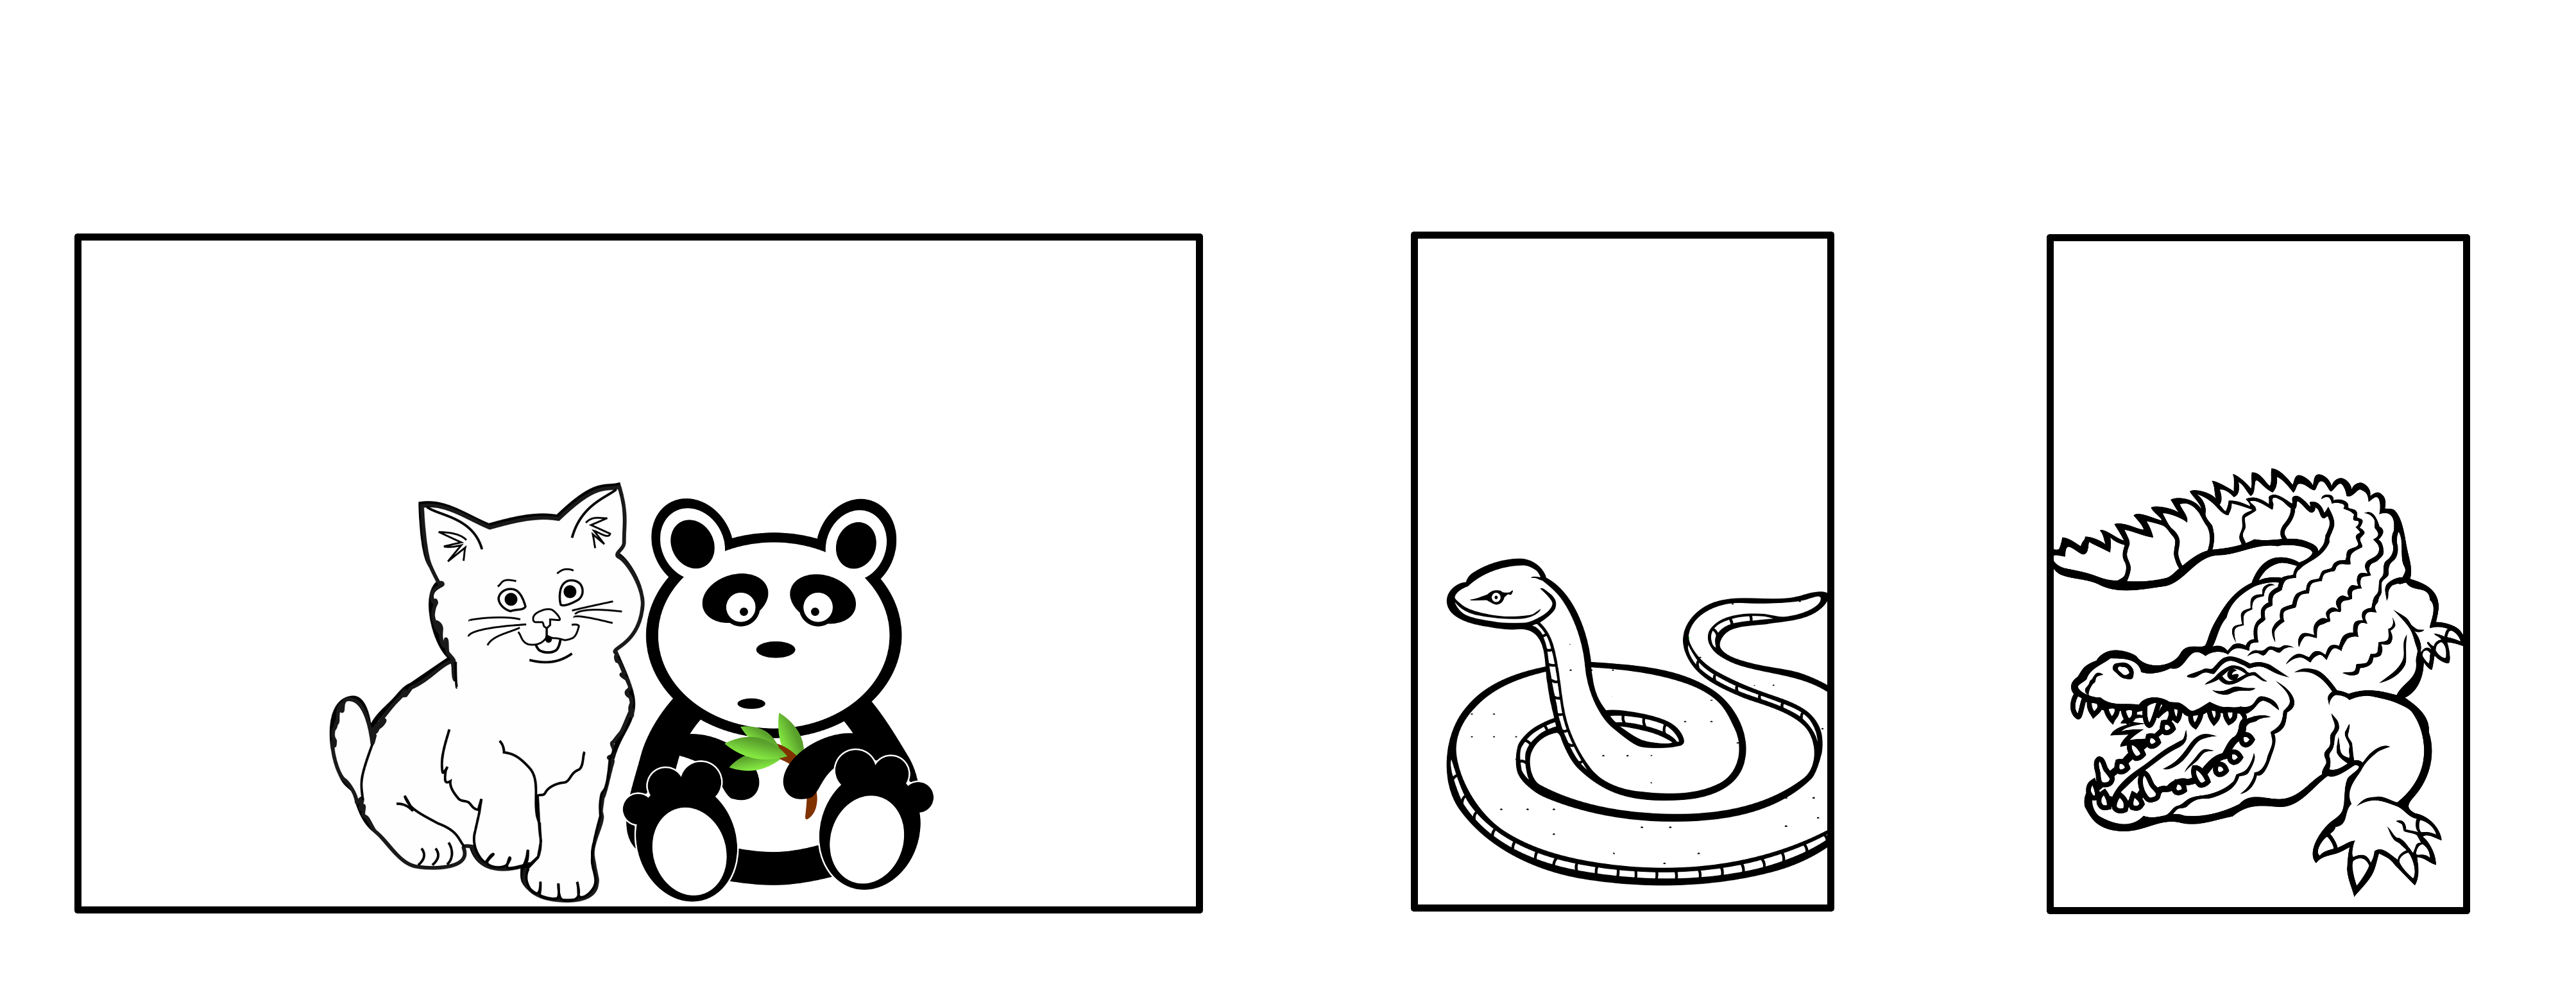
\includegraphics[width=1\textwidth]{Illustrations/doors_animals_panda.png}
\end{figure} 

\newpage
\section{Picture Sources}
\begin{itemize}
\item Figure \ref{fig:mysterious_doors}: \href{https://flic.kr/p/aQUzkH}{``Deciding Which Door to Choose 2''} by \href{https://www.flickr.com/photos/59632563@N04/}{Vic} is licensed under \href{https://creativecommons.org/licenses/by/2.0/}{CC BY 2.0}
\item Figures \ref{fig:one_ordering} and \ref{fig:different_ordering} are composed of the following images:
	\begin{itemize}
	\item \href{http://animalsclipart.com/contour-drawing-of-little-kitten-cat/}{``Contour Drawing of Little Kitten Cat''} by Brian Ramirez is licensed under \href{https://creativecommons.org/licenses/by/4.0/}{CC BY 4.0}
	\item \href{http://animalsclipart.com/grizzly-bear-stencil-clipart/}{``Grizzly Bear Stencil Clipart''} by Ryan Sanders is licensed under \href{https://creativecommons.org/licenses/by/4.0/}{CC BY 4.0}
	\item \href{http://animalsclipart.com/outline-snake-clipart-in-black-and-white/}{``Outline Snake Clipart in Black and White''} by Agnes Farmer is licensed under \href{https://creativecommons.org/licenses/by/4.0/}{CC BY 4.0}
	\item \href{http://animalsclipart.com/stencil-design-of-wild-crocodile-in-black-and-white/}{``Stencil Design of Wild Crocodile in Black and White''} by Robert Carter is licensed under \href{https://creativecommons.org/licenses/by/4.0/}{CC BY 4.0}
	\end{itemize}
\item Figure \ref{fig:CMBH} is composed of the following images:
	\begin{itemize}
	\item \href{http://animalsclipart.com/cat-outline-logo-drawing-design/}{``Cat Outline Logo Drawing Design''} by Carl Powell is licensed under \href{https://creativecommons.org/licenses/by/4.0/}{CC BY 4.0}
	\item \href{http://animalsclipart.com/monkey-outline-clipart-in-black-and-white/}{``Monkey Outline Clipart in Black and White''} by Paul Foster is licensed under \href{https://creativecommons.org/licenses/by/4.0/}{CC BY 4.0}
	\item \href{http://animalsclipart.com/outline-bear-drawing/}{``Outline Bear Drawing''} by Emily Bennett is licensed under \href{https://creativecommons.org/licenses/by/4.0/}{CC BY 4.0}
	\item \href{http://animalsclipart.com/drawing-outline-of-horse-in-black-and-white/}{``Drawing Outline of Horse in Black and White''} by Frank Lewis is licensed under \href{https://creativecommons.org/licenses/by/4.0/}{CC BY 4.0}
	\end{itemize}
\item Figures \ref{img:neighborhood_graph}, \ref{img:PRISM}, \ref{img:UML}, \ref{img:binarysearchtree_example_pf}, \ref{img:binarysearchtreelimiteddepth_example_pf}, \ref{img:random_tree}, \ref{img:graph_example_pf} and \ref{img:supermodel_merge} were made/are screenshots by me.
\item Figure \ref{img:plus_panda} is composed of the following images:
	\begin{itemize}
	\item \href{http://animalsclipart.com/contour-drawing-of-little-kitten-cat/}{``Contour Drawing of Little Kitten Cat''} by Brian Ramirez is licensed under \href{https://creativecommons.org/licenses/by/4.0/}{CC BY 4.0}
	\item \href{http://animalsclipart.com/panda-bear-clipart-with-branch-in-hand/}{``Panda Bear Clipart with Branch in Hand''} by Patricia Wood is licensed under \href{https://creativecommons.org/licenses/by/4.0/}{CC BY 4.0}
	\item \href{http://animalsclipart.com/outline-snake-clipart-in-black-and-white/}{``Outline Snake Clipart in Black and White''} by Agnes Farmer is licensed under \href{https://creativecommons.org/licenses/by/4.0/}{CC BY 4.0}
	\item \href{http://animalsclipart.com/stencil-design-of-wild-crocodile-in-black-and-white/}{``Stencil Design of Wild Crocodile in Black and White''} by Robert Carter is licensed under \href{https://creativecommons.org/licenses/by/4.0/}{CC BY 4.0}
	\end{itemize}
\item The reproduction of figures \ref{fig:Equidistant equiintense information injections into a system with memory strength 1} and \ref{fig:Equidistant equiintense information injections into a system with memory strength 2} was generously allowed by authors of \cite{Yffelti.2016}.
\end{itemize}

\bibliography{literature}
%\section{List of Used Software}

\end{document}
